\documentclass[11pt,a4paper,leqno]{report}
\usepackage{tikz-cd}
\usepackage{tikz}
%\usepackage[german]{babel}
\usepackage{amsmath}
\usepackage{amsthm}
\usepackage{amssymb}
\usepackage{float}
\usepackage{amsfonts}
\usepackage{hyperref}
\usepackage{lmodern}
%\usepackage{makeidx}
%\usepackage{graphicx}
%\graphicspath{{pics/}}
\usepackage{svg}
\usepackage{amsmath}
\usepackage{delarray}
\makeatletter
\renewcommand*\env@matrix[1][*\c@MaxMatrixCols c]{%
	\hskip -\arraycolsep
	\let\@ifnextchar\new@ifnextchar
	\array{#1}}
\makeatother
\newcommand{\eps}{\varepsilon}
\newcommand{\R}{\mathbb{R}}
\newcommand{\C}{\mathbb{C}}


%%%%%%%%%%% REST %%%%%%%%%%%%%%%%%%%%%%%%%%%%%%%%%%%%

\DeclareMathOperator{\dom}{dom}
\DeclareMathOperator{\ran}{ran}
\newcommand{\re}{\mathrm{Re}}
\newcommand{\im}{\mathrm{Im}}

\newcommand{\ul}{\underline}
\newcommand{\I}{\mathrm{i}}
\newcommand{\E}{\mathrm{e}}

%\makeindex
%\setlength{\parindent}{0em} 


\newtheorem{theorem}{Theorem}[chapter]
\newtheorem{proposition}{Satz}[chapter]
\newtheorem{lemma}[theorem]{Hilfssatz}
\newtheorem{definition}[theorem]{Definition}
\newtheorem{corollary}[theorem]{Folgerung}
\newtheorem{remark}[theorem]{Bemerkung}

\renewcommand{\figurename}{Abbildung}
\numberwithin{equation}{chapter}



\usepackage{listings}
\lstset{basicstyle=\ttfamily}
\lstset{literate=%
	{\"o}{{\"O}}1
	{\"a}{{\"A}}1
	{\"u}{{\"U}}1
	{\"u}{{\"u}}1
	{\"a}{{\"a}}1
	{\"o}{{\"o}}1
}
\renewcommand{\chaptername}{Kapitel}
\renewcommand{\contentsname}{Inhaltsverzeichnis}
\renewcommand{\proofname}{Beweis}
\begin{document}


\begin{titlepage}

\vspace*{5cm}
\begin{center}
\rule{\linewidth}{0.5mm} \\[0.4cm]
{ \Huge \bfseries Eine Spielmodell des Elektromagnetismus auf planaren Graphen} \\[0.2cm]
\rule{\linewidth}{0.5mm} \\[3.5cm]
\begin{minipage}[t]{0.4\textwidth}
\begin{flushleft} \large
\emph{Author:}\\
Oliver \textsc{Sko\v{c}ek} \\[4cm]
\small

\end{flushleft}

\end{minipage}
\begin{minipage}[t]{0.4\textwidth}

\end{minipage}
 
% Bottom of the page

 
\end{center}
 
\end{titlepage}

%\maketitle


%\renewcommand{\contentsname}{Contents}

\tableofcontents

\markboth{Contents}{Contents}

\vfill


\chapter*{Einf\"uhrung}
Die Absicht dieser Arbeit ist es ausgehend von der Theorie elektrischer Netzwerke eine Theorie elektromagnetischer Ph\"anomene in der Ebene zu entwickeln. Dabei soll kein Kontinuums\"ubergang gemacht werden sondern allein mit planaren Graphen gearbeitet werden. Zu diesem Zwecke werden einige grundlegende Begriffe der Graphentheorie eingef\"uhrt. Darauf aufbauened werden dann im zweiten Kapitel Funktionnenr\"aume auf diesen Graphen definiert und analog zur mehrdimensionalen Analysis wird eine Theorie mit Analogien zum gewohnten Gradienten, der Divergenz und dem Rotor vorgestellt. Abgeschlossen wird diese Theorie durch ein zum de Rham Komplex analoges Theorem. \\Im dritten Kapitel wird dann ein verallgemeinertes Poissonproblem vorgestellt, dass direkt verwendet werden kann um Widerstandsnetzwerke zu l\"osen. Dies zeigt, dass viele Analogien zwischen dem Problem der Widerstandsnetzwerke und dem Poissonproblem der Elektrostatik existieren.\\
Im vierten Kapitel wird dann eine Version der Maxwell-Gleichungen auf planaren Graphen vorgestellt und zwei wichtige Eigenschaften, Energieerhaltung und Ladungserhaltung behandelt.
Im darauffolgenden Kapitel werden die Maxwellgleichungen in Potentialformulierung vorgestellt und ihre Symmetrie die Eichtransformation vorgestellt.
Im Kapitel "kanonische Quantisierung" wird dann der Sprung von einer klassischen Theorie in eine Quantentheorie gemacht und die Schr\"odingergleichung elektromagnetischer Felder konstruiert.

\chapter{Planare Graphen}
	Ein Graph besteht aus Ecken $V$ und Kanten $E$. Die Ecken und Kanten stehen in Beziehung zueinander. Man sagt eine Kante \emph{verbindet} zwei Ecken. Wir wollen nur solche Graphen betrachten, deren Kanten jeweils zwei unterschiedliche Ecken verbinden.
\begin{figure}[H]
	\begin{center}
		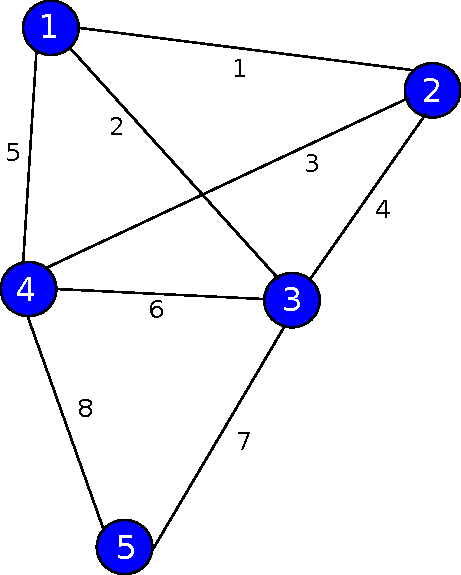
\includegraphics[scale=0.4]{Abbildungen/graph_1.pdf}
		\caption{Beispiel Graph.}
	\end{center}
\end{figure}
\noindent
	Die Beziehung zwischen Ecken und Kanten kann durch eine Matrix dargestellt werden. Der vertikale Index der Matrix steht f\"ur die Kanten und der horizontale Index steht f\"ur die Ecken. Die Matrix ist Eins falls die Kante die Ecke mit einer anderen Ecke verbindet und sonst Null. Diese Matrix nennt man die \textbf{Inzidenzmatrix} des Graphen.\\
	Als Beispiel betrachte die Inzidenzmatrix des Graphen in Abbildung 2.1.
	\begin{center}
		\begin{tabular}{c c c c c}
			1 & 1 & 0 & 0 & 0\\
			1 & 0 & 1 & 0 & 0\\
			0 & 1 & 0 & 1 & 0\\
			0 & 1 & 1 & 0 & 0\\
			1 & 0 & 0 & 1 & 0\\
			0 & 0 & 1 & 1 & 0\\
			0 & 0 & 1 & 0 & 1\\
			0 & 0 & 0 & 1 & 1\\
		\end{tabular} 
	\end{center}
	Im Grunde interessieren wir uns nicht f\"ur die spezielle Realisierung von Ecken und Kanten, sondern f\"ur die Verbindungsstruktur, die genau durch die Inzidenzmatrix festgelegt wird. Dies legt folgende Definition nahe.
\begin{definition}
	Ein \textbf{Graph} ist eine Matrix (Inzidenzmatrix) deren Zeilensumme zwei ist. Zwei Graphen mit Inzidenzmatrizen $X$ und $Y$ sind gleich falls man $X$ aus $Y$ durch Vertauschung von Zeilen und Spalten erhalten kann.
\end{definition}
\begin{remark}
	Alternativ kann ein Graph auch durch eine Adjazenzmatrix definiert werden. Eine solche Matrix ist quadratisch und beide Indizes stehen f\"ur die Ecken des Graphen. Die Adjazenzmatrix ist eins falls die Ecken durch eine Kante verbunden sind und sonst Null. Als Beispiel die Adjazenzmatrix unseres Beispielgraphen.
	\begin{center}
	\begin{tabular}{c c c c c}
		0 & 1 & 1 & 1 & 0\\
		1 & 0 & 1 & 1 & 0\\
		1 & 1 & 0 & 1 & 1\\
		1 & 1 & 1 & 0 & 1\\
		0 & 0 & 1 & 1 & 0\\
	\end{tabular} 
\end{center}
	Der Nachteil der Adjazenzmatrix ist, dass sie keine Mehrfachkanten zwischen zwei Ecken zul\"asst.
\end{remark}
\noindent
Manchmal ist es notwendig \"uber Teile von Graphen zu sprechen. Hierzu dient das Konzept des Teilgraphen. Ein Teilgraph eines Graphen $G$ ist ein Graph, den man durch entfernen von Ecken und Kanten aus $G$ erh\"alt. Bedenke dabei, dass mit jeder Ecke auch alle diese Ecke verbindenten Kanten entfernt werden m\"ussen.
\begin{definition}
	Sei $G$ ein Graph mit Inzidenzmatrix $X$ und $H$ ein Graph mit Inzidenzmatrix $Y$, dann ist $G$ ein \textbf{Teilgraph} von $H$, falls man die Matrix $X$ durch entfernen von Zeilen oder Spalten aus der Matrix $Y$ erhalten kann.
\end{definition}
\noindent
Betrachten wir hierzu einen Teilgraph des Beispielgraphen.
\begin{figure}[H]
	\begin{center}
		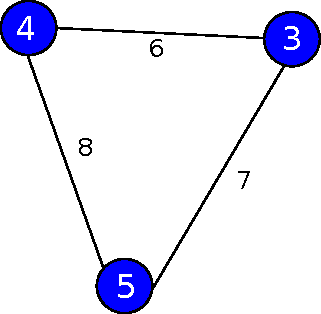
\includegraphics[scale=0.4]{Abbildungen/graph_1_teil.pdf}
		\caption{Teilgraph des Beispielgraphs.}
	\end{center}
\end{figure}
\noindent
Die zugeh\"orige Inzidenzmatrix erhalten wir indem wir die ersten beiden Spalten entfernen und anschlie{\ss}end alle Zeilen, deren Summe ungleich zwei ist. 
\noindent
Das Resultat ergibt dann f\"ur kannten 4, 7 und 8 folgende Inzidenz mit den Ecken 3, 4 und 5.
	\begin{center}
	\begin{tabular}{c c c}
		1 & 1 & 0\\
		1 & 0 & 1\\
		0 & 1 & 1\\
	\end{tabular} 
\end{center}
Eine spezielle Art von Teilgraph erh\"alt man, wenn man eine Teilmenge $U$ der Ecken fixiert und alle Kanten aus dem Graphen entfernt, die eine nicht in der Teilmenge $U$ enthaltene Ecke verbinden. Man nennt so einen Graph den durch die Menge $U$ \textbf{induzierten Teilgraph}. Der Teilgraph in Abbildung 2.2 ist ein solches Beispiel. Es ist der durch $U =\{3, 4, 5\}$ induzierte Teilgraph des Beispielgraphen.
\begin{definition}
	Sei $G$ ein Graph und $n$ eine nat\"urliche Zahl, dann nennt man eine Folge von Ecken $(x_0, x_1,\dots,x_n)$ f\"ur die gilt, dass auf einander folgende Ecken immer durch eine Kante verbunden sind, einen \textbf{Pfad} auf $G$. Falls $x_0 = x_n$ gilt, nennt man dies einenen \textbf{geschlossenen Pfad}. Falls zus\"atzlich bis auf $x_0$ und $x_n$ keine Ecke mehrfach vorkommt, nennt man den Pfad \textbf{einfach geschlossen}.\\
	Man nennt $G$ \textbf{zusammenh\"angend}, falls man von jeder Ecke von $G$ jede andere Ecke \"uber einen Pfad erreichen kann. Sei weiters $k\in\mathbb{N}$, dann sagt man ein Graph ist \textbf{$k$-fach zusammen\-h\"angend}, falls man $k - 1$ beliebige Kanten entfernen k\"onnte und der resultierende Graph immer noch zusammenh\"angend w\"are.
\end{definition}
\noindent
Alle Graphen werden von hier an als zusammenh\"angend angenommen. Allgemein l\"asst sich jeder Graph als Ansammlung von zusammenh\"angenden Teilgraphen darstellen, wodurch diese Annahme im Sinne einer Vereinfachung gerechtfertigt wird.
\begin{definition}
	Ein Graph hat eine \textbf{planare Darstellung} wenn man den Graph auf einem Blatt Papier zeichnen kann, indem man f\"ur jede Ecke einen Punkt zeichnet und f\"ur jede Kante einen Strich zwischen den Eck-Punkten, die sie verbinden soll, ohne das sich dabei zwei Striche kreuzen.
\end{definition}
\noindent
	Der Graph aus Abbildung 2.1 hat eine planare Darstellung. Um dies zu sehen muss man nur die Position von Ecke Nummer 2 ver\"andern.
\begin{figure}[H]
	\begin{center}
		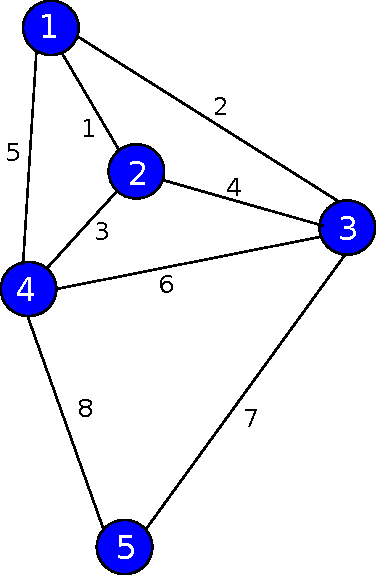
\includegraphics[scale=0.4]{Abbildungen/graph_1_planar.pdf}
		\caption{Beispiel Graph (planar).}
	\end{center}
\end{figure}
\noindent
	Im Allgemeinen gibt es mehrere Wege wie ein bestimmter Graph gezeichnet werden kann. Es gibt sogar f\"ur ein und denselben Graphen oft mehrere planare Darstellungen.
\begin{figure}[H]
	\begin{center}
		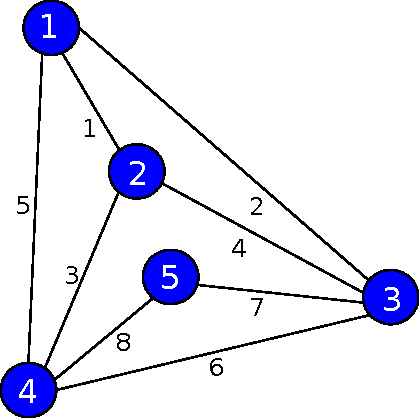
\includegraphics[scale=0.4]{Abbildungen/graph_1_planar2.pdf}
		\caption{Beispiel Graph (planar) alternativ.}
	\end{center}
\end{figure}
\noindent
Es ist also zus\"atzliche Information notwendig um eine planare Darstellung eindeutig festzulegen. Diese zus\"atzliche Information kann \"uber die Fl\"achen aus denen sich die planare Darstellung zusammensetzt gegeben werden.\\
\begin{definition}
	Sei $G$ ein Graph, dann nennt man $G$ einen \textbf{Zyklus} oder \textbf{zyklisch}, falls jede Ecke von $G$ mit genau zwei Kanten verbunden ist.
\end{definition}
\noindent
Betrachten wir eine der planaren Darstellungen des Beispielgraphen. Eine \textbf{Fl\"ache} ist hier ein Zyklus, der keine Ecke einschlie\ss{}t.
\begin{figure}[H]
	\begin{center}
		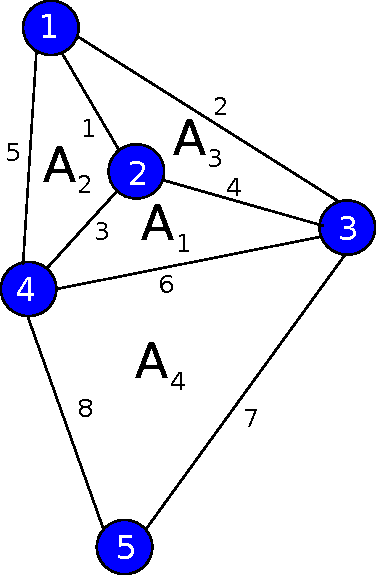
\includegraphics[scale=0.3]{Abbildungen/graph_1_planar_flach.pdf}
		\caption{Beispiel Graph (planar) mit Fl\"achen.}
	\end{center}
\end{figure}
\noindent
\begin{remark}
	Sei $G$ ein Graph und $\{A_1, A_2, \dots, A_n\}$ eine Menge von zyklischen induzierten Teilgraphen, sodass jede Kante von $G$ in maximal zwei der Zyklen vorkommt und jede Ecke von $G$ in mindestens einem der Zyklen vorkommt, dann gibt es eine eindeutige planare Darstellung des Graphen $G$, dessen Fl\"achen genau die $\{A_1, A_2, \dots, A_n\}$ sind.  
\end{remark}
\begin{definition}
	Ein planarer Graph $G=(g, f)$ ist ein Graph $g$ und eine Menge $f$ von Zyklen aus $g$ wie in Bemerkung 1.6. beschrieben. Sei weiters $e$ eine Kante von $g$, dann sagt man $e$ liegt am \textbf{Rand} des Graphen wenn $e$ genau einmal in einer Fl\"ache vorkommt. Der Teilgraph, der genau die am Rand liegenden Kanten enth\"alt nennt man den \textbf{Rand des Graphen}.
\end{definition}
\noindent
Die in Bemerkung 1.6. beschriebene Struktur legt ein mit planaren Graphen eng verkn\"upftes Konzept nahe. Jede Kante des Graphen ist entweder ein Bindeglied zwischen zwei Fl\"achen oder es liegt am Rand des Graphen. Die am Rand liegenden Kanten k\"onnen wiederum als Bindeglied mit der den Graphen umgebenden Fl\"ache, genannt $A_{\infty}$, angesehen werden und somit haben wir das Konzept des dualen Graphen entdeckt.
\begin{definition}
	Es sei $G$ ein planarer Graph, dann kann man einen neuen Graphen, den \textbf{dualen Graph} $G^D$, konstruieren, dessen Kanten mit denen von $G$ \"ubereinstimmen, aber dessen Ecken die Fl\"achen von $G$ zusammen mit der umgebenden Fl\"ache sind, also $V=\{A_1, A_2, \dots, A_n, A_\infty \}$. F\"ur eine gegebene Kante $e$ und Ecke des dualen Graphen $v\in V$ ist die Inzidenzmatrix Eins falls $e$ die Fl\"ache $v$ begrenzt und sonst Null.
\end{definition}
\noindent
Betrachte den dualen Graph des planaren Graphen aus Abbildung 1.5. Beachte die doppelte Kante zwischen Ecke $A_4$ und Ecke $A_\infty$. 
\begin{figure}[H]
	\begin{center}
		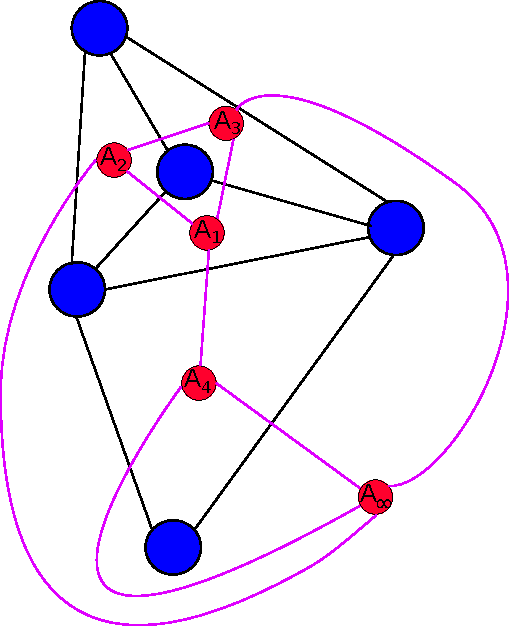
\includegraphics[scale=0.4]{Abbildungen/graph_1_dual.pdf}
		\caption{Dualer Graph des Beispielgraphen.}
	\end{center}
\end{figure}
\noindent
Die blauen Ecken symbolisieren die Ecken des Ausgangsgraphen, während die roten Ecken die Ecken des dualen Graphen darstellen. Die Platzierung von $A_\infty$ ist beliebig gew\"ahlt. Offensichtlich bestimmt diese Wahl, welcher der Ecken des Ausgangsgraphen die umgebende Fl\"ache des dualen Graphen darstellt.
\begin{remark}
	Der duale Graph $G^D$ ist immer auch fast ein planarer Graph, denn jede Ecke von $G$ kann mit einem Zyklus in $G^D$ identifiziert werden, somit bleibt aber offen welche dieser Zyklen, die umgebende Fl\"ache ist. Dies ist insbesondere von Bedeutung wenn man den dualen Graphen des dualen Graphen, den so genannten \textbf{bidualen Graphen} bildet. Um eine eindeutige Zuordnung zu erzwingen muss immer einer der Ecken ausgezeichnet werden oder man verzichtet auf die planare Darstellung und arbeitet mit Polyedern. 
\end{remark}
\noindent
Bislang wurden nur "ungerichtete Graphen" behandelt, also solche deren Kanten keine ausgzeichnete Beziehung mit der einen oder der anderen durch sie verbundenen Ecke haben. Graphen, deren Kanten eine solche Orientierung aufweisen, nennt man "gerichtete Graphen" und eine Adjazenzmatrix ist ein praktisches Weg um solche Strukturen zu beschreiben. Im Gegensatz zur Adjazenzmatrix eines ungerichteten Graphen wird im gerichteten Fall, einfach die Forderung nach Symmetrie der Matrix weggelassen.
\begin{definition}
	Jeder planare Graph kann mit einer \textbf{Orientierung} \\ausgestattet werden, dies ist eine Funktion, die jeder Kante eine der Ecken zuordnet, die durch sie verbunden wird. Man stelle sich vor jede Kante ist ein Pfeil und die Orientierung gibt an auf welche Ecke sie zeigt. Man unterscheidet entsprechend eine \textbf{Spitzefunktion} $x\mapsto p(x)$, welche die Ecke zuordnet, die an der Pfeilspitze liegt und die \textbf{Schaftfunktion} $x\mapsto q(x)$, welche die andere Ecke zuordnet.
\end{definition}
\begin{figure}[H]
	\begin{center}
		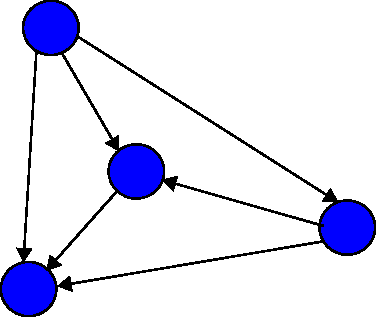
\includegraphics[scale=0.4]{Abbildungen/graph_1_orient.pdf}
		\caption{Graph mit Orientierung.}
	\end{center}
\end{figure}
\noindent
 Zu einem gegebenen Graph gibt es $2^{|E|}$ M\"oglichkeiten, wobei $E$ die Kanten\-menge ist, einen gegebenen Graph mit einer Orientierung auszustatten und ihn hierdurch zu einem gerichteten Graphen zu erheben.
 \begin{remark}
 	Jede Orientierung auf einem planaren Graph $G$, bestimmt eindeutig eine zu ihr \textbf{duale Orientierung} auf dem dualen Graph. Sei hierzu $A$ eine Fl\"ache des planaren Graphen $G$, also ein induzierter Teilgraph, der ein Zyklus ist, und $e$ eine Kante des Graphen, die auch in $A$ liegt, dann setzen wir die Spitzenfunktion $p_D$ der dualen Orientierung $p_D(e) = A$, falls $e$ im planaren Graph $G$ im Uhrzeigersinn bez\"uglich zu $A$ orientiert ist.
 \end{remark}
\begin{figure}[H]
	\begin{center}
		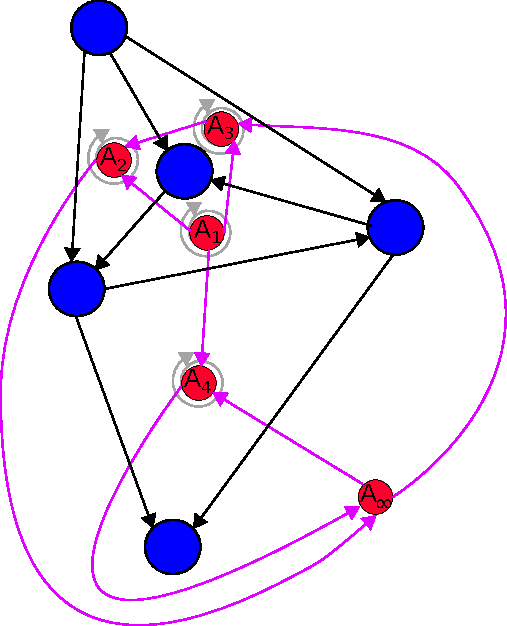
\includegraphics[scale=0.4]{Abbildungen/graph_1_dual_orient.pdf}
		\caption{Orientierung und duale Orientierung.}
	\end{center}
\end{figure}
\noindent

\chapter{Funktionenr\"aume und Operatoren}
Im letzten Kapitel wurden Graphen mit zus\"atzlicher Struktur beschrieben, nämlich planare Graphen und das Konzept des dualen Graphen. In diesem Kapitel sollen die drei Arten von Funktionen auf planaren Graphen und Operatoren, die diese Funktionen aufeinander abbilden vorgestellt werden.
\begin{definition}
	Sei $G$ ein planarer Graph und $G^D$ sein dualer Graph, des weiteren sei $V$ die Menge der Ecken, $E$ die Menge der Kanten und $A$ die Menge der Fl\"achen (inklusive umgebende Fl\"ache), dann unterscheiden wir drei verschiedene (endlichdimensionale) Funktionenr\"aume auf dieser Struktur, den Raum der Kantenfunktionen $\mathfrak{K}=\{f|f: E\rightarrow\mathbb{R}\}$, den Raum der Eckfunktionen $\mathfrak{E}=\{f|f: V\rightarrow\mathbb{R}\}$ und den Raum der Fl\"achenfunktionen $\mathfrak{F}=\{f|f: A\rightarrow\mathbb{R}\}$. Die analogen komplexen Funktionenr\"aume werden abgek\"urzt als $\mathfrak{F}_\mathbb{C}$,$\mathfrak{E}_\mathbb{C}$ und $\mathfrak{K}_\mathbb{C}$.
\end{definition}
\noindent
Es gibt eine nat\"urliche Beziehung zwischen diesen drei R\"aumen. 
\begin{definition}
	Sei $G$ ein Graph, $f\in\mathfrak{E}(G)$ eine Eckfunktion auf $G$, seien weiters $p$ und $q$ die Spitzefunktion und Schaftfunktion einer Orientierung auf $G$, dann nennt man $grad(f)\in\mathfrak{K}(G)$ definiert durch 
	$$grad(f)(e) = f(p(e)) - f(q(e))$$ 
	f\"ur eine beliebige Kante $e$ den Gradienten von $f$.
\end{definition}
\begin{definition}
	Sei $G$ ein Graph, $f\in\mathfrak{K}(G)$ eine Kantenfunktion auf $G$, seien weiters $p$ und $q$ die Spitzefunktion und Schaftfunktion einer Orientierung auf $G$, dann nennt man $div(f)\in\mathfrak{E}(G)$, definiert durch: 
	$$div(f)(x) = \sum_{\acute{e}\in E, q(\acute{e})=x}f(\acute{e}) -\sum_{e\in E, p(e)=x}f(e)$$
	f\"ur eine beliebige Ecke $x$ die Divergenz von $f$.
\end{definition}
\noindent
	Der Gradient hebt eine Eckfunktion auf die Kanten, und die Divergenz eine Kantenfunktion auf die Ecken. Der Graph $G$ und der duale Graph $G_D$ haben dieselben  Kantenfunktionen, daher bildet dieser Raum eine Verbindung zwischen Gradient und Divergenz des Graphen und des dualen Graphen. Der Gradient und die Divergenz des dualen Graphen werden durch $grad_D$ respektive $div_D$ symbolisiert. Falls eine Kantenfunktion als Fluss interpretiert wird, entspricht die Divergenz der Kantenfunktion dem Nettofluss von den Ecken weg.
\begin{proposition}
		Sei $G$ ein planarer Graph mit Orientierung, dann sind der Gradient und die Divergenz lineare Operatoren und es gilt:
		$$div = -grad^T$$
		wobei sich die Adjunktion auf das Standardskalarprodukt bezieht.
\end{proposition}
\begin{proof}
Sei $u\in\mathfrak{E}(G)$ und $v\in \mathfrak{K}$, dann schreiben wir das Skalarprodukt:
$$\langle v, \text{grad}(u)\rangle_\mathfrak{K} = \sum_{x\in E} v(x) * (u(p(x) - u(q(x)))) = $$
$$\sum_{x\in E} v(x) * u(p(x)) - \sum_{x\in V} v(x) * u(q(x))=$$
$$\sum_{e\in V} u(e) * \sum_{j\in E, p(j)=e}v(j) - \sum_{e\in V} u(e) * \sum_{j\in E, q(j)=e}v(j) =$$
$$-\langle \text{div}(v), u\rangle_\mathfrak{E}$$
\end{proof}
\begin{definition}
	Sei $G$ ein planarer Graph mit Orientierung und $f\in\mathfrak{K}(G)$, $(x_i)_{i=1}^n$ ein Pfad auf $G$, $(e_i)_{i=1}^{n-1}$ die Folge der Kanten, die f\"ur jedes $1\leq i \leq n-1$ $x_i$ und $x_{i+1}$ verbinden und es sei $\sigma_i$ f\"ur jedes $1\leq i \leq n-1$ gleich $-1$ falls $p(e_i)=x_i$ ist und sonst $+1$, dann nennt man die Summe
	$$ \sum_{i=1}^{n-1} \sigma_i f(e_i)$$
	die \textbf{Pfadsumme.}
\end{definition}
\begin{proposition}
	Sei $G$ ein planarer Graph mit Orientierung, $f\in\mathfrak{K}(G)$ sodass $\text{div}_D(f)=0$, dann gilt dass f\"ur jeden geschlossenen Pfad in $G$ die Pfadsumme gleich Null ist.
\end{proposition}
\begin{proof}
Zu allererst reicht es einfach geschlossene Pfade zu betrachten. Diese Einschränkung ist zul\"assig weil sich f\"ur alle anderen geschlossenen Pfade die Pfadsumme sich als Summe solcher einfach geschlossenen Pfade schreiben l\"asst.\\
\\
Jeder einfach geschlossene Pfad zerteilt den Graph in zwei Teilgraphen, sodass die Vereinigung der Teilgraphen ganz $G$ ist und der Durchschnitt nur den geschlossenen Pfad enth\"alt. Jener Teilgraph, der keinen Teil des Randes von $G$ enth\"alt ist der innere Graph.\\
\\
Sei $f\in\mathfrak{K}(G)$, dann gilt f\"ur jeden Zyklus in $G$, dass falls er als Pfad gegen den Uhrzeigersinn orientiert geschrieben wird, die Pfadsumme gleich dem Wert von $\text{div}_D$ ist.\\
\\
Sein nun $(x_i)_{i=1}$ ein einfach geschlossener Pfad, dann k\"onnen wird die Pfad- summe als Summe \"uber alle Zyklen des zugeh\"origen inneren Graphen schreiben, da die Pfade \"uber die Zyklen immer als gegen den Uhrzeigersinn orientiert angenommen werden, heben sich alle Kantenwerte auf, die nicht zum Pfad $(x_i)_{i=1}$ geh\"oren.
Da $\text{div}_D(f)=0$ ist, ist somit auch die Pfadsumme gleich Null.
\end{proof}
\noindent
	Es besteht eine Analogie der hier definierten Operatoren zu den Differential\-operatoren der Vektoranalysis. Interessanterweise entspricht die duale Divergenz der Rotation. Die Analogie untermauernd kann man folgendes Theorem formulieren.
\begin{theorem}[Der de Rham Komplex]
	Die Operatoren $grad$, $div$, $grad_D$ und $div_D$ erf\"ullen folgende exakte Sequenzen, daher das Bild der Abbildungen entspricht dem Kern der nachfolgenden Abbildung. Beachte, dass $\mathbb{R}$ in den Formeln f\"ur die dem entsprechenden Raum zugeh\"origen konstanten Funktionen steht.
\begin{equation}
	\mathbb{R}\longrightarrow\mathfrak{E}(G) \overset{grad}{\longrightarrow}\mathfrak{K}(G) \overset{div_D}{\longrightarrow}\mathfrak{F}(G)/\mathbb{R}\longrightarrow 0
\end{equation}
\begin{equation}
	\mathbb{R}\longrightarrow\mathfrak{F}(G) \overset{grad_D}{\longrightarrow}\mathfrak{K}(G) \overset{div}{\longrightarrow}\mathfrak{E}(G)/\mathbb{R}\longrightarrow 0
\end{equation}
\end{theorem}
\begin{proof}[Beweis de Rham Komplex]
	Es gen\"ugt Gleichung 2.1 in Theorem 2.4 zu beweisen, da 2.2 durch Anwendung von 2.1 auf den dualen Graphen folgt.\\
	\\
	\textbf{Erste zu beweisende Aussage:} Der Kern von $\text{grad}$ ist genau der Raum der konstanten Eckfunktionen.\\
	\\
	Da $G$ zusammenh\"angend ist und da $\text{grad}$ an einer Kante nur Null sein kann wenn beide Ecken, welche die Kante verbindet, den selben Wert haben, ist $\text{grad}(f)$ genau dann Null wenn $f$ konstant ist.\\
	\\
	\textbf{Zweite zu beweisende Aussage:} Das Bild von $\text{grad}$ ist genau der Kern von $\text{div}_D$.\\
	\\
	Sei $a$ ein Zyklus von $G$, und $(x_i)_{i=1}^k$ ein Pfad der die Ecken des Zyklus gegen den Uhrzeigersinn durchl\"auft und $f\in\mathfrak{E}$, dann gilt:
	$$div_D(\text{grad}(f)) = \sum_{i=1}^{k-1} \sigma(i) * \overbrace{\sigma(i) * (f(x_{(i+1) \text{ mod } k})-f(x_{i  \text{ mod } k}))}^{\text{grad}}$$
	Da ja $k \text{ mod }k=0$ gilt, kommt in der Summe jeder Wert von $f$ genau einmal mit positiven und einmal mit negativen Vorzeichen vor. Daher die Summe ist gleich Null.\\
	\\
	Es fehlt noch zu zeigen, dass jedes Element im Kern von $\text{div}_D$ auch im Bild von $\text{grad}$ ist.\\
	\\
	Sei $f$ eine Kantenfunktion, sodass gilt $\text{div}_D(f)=0$, dann gilt wegen dem Satz 2.2, dass f\"ur beliebige Ecken $a, b\in V$ gilt, dass die Pfadsummen f\"ur alle Pfade, die in $a$ starten und in $b$ enden, gleich sind.\\
	\\
	W\"ahlen wir nun eine beliebige Ecke $x_0$, weil $G$ zusammenh\"angend ist, k\"onnen wir von $x_0$ zu jeder Ecke in $G$ einen Pfad bilden um $F\in\mathfrak(E)(G)$ zu definieren, sodass f\"ur jede Ecke $x$ $F(x)$ gleich der Pfadsumme eines Pfades von $x_0$ nach $x$ hat. Dies ist ja eindeutig. Es gilt nun $\text{grad}(F) = f$.
	\\
	\\
	\textbf{Die letzte zu beweisende Aussage:} Das Bild von $\text{div}_D$ ist genau das orthogonale Komplement der konstanten Fl\"achenfunktionen.\\
	\\
	Wegen des Satzes 2.1 und der ersten Aussage in diesem Beweis folgt die Aussage.
\end{proof}
\noindent
\chapter{Das Poisson Problem}
Ein klassisches Problem der Theorie elektrischer Netzwerke sowie der Elektrostatik ist das (verallgemeinerte) Poissonproblem. Dieses Problem wird hier in einigen seiner Facetten vorgestellt und basierend auf der bisher behandelten Graphentheorie formuliert und gel\"ost.
\paragraph{Das verallgemeinerte Poisson Problem}
Sei $G$ ein Graph, $\partial$ eine Teilmenge der Ecken, $r$ eine positive Kantenfunktion und $f$ und $g$ Eckfunktionen, dann wird eine Eckfunktion $u$ gesucht sodass gilt:

\begin{align}
	-div(r * grad(u))(x) = f(x)\text{  falls } x\notin \partial\\
	u(x) = g(x)\text{  falls } x\in \partial
\end{align}
Die Bedingung 3.2 ist motiviert durch Randwertprobleme aus der Theorie der partiellen Differential\-gleichungen.
\begin{definition}
	Sei $G$ ein planarer Graph mit Orientierung, $r$ eine positive Kantenfunktion, dann nennt man $\Delta_r$, definiert durch 
	$$\Delta_r(u) = -div(r * grad(u))\text{ falls }u\in\mathfrak{E}(G)$$
	den \textbf{$r$-gewichteten Laplace} Operator
\end{definition}
\paragraph{Die Formulierung f\"ur elektrische Netzwerke}Gegeben ein Netzwerk(Graph) bestehend aus Spannungsquellen, Stromquellen und linearen Komponenten (elektrische Widerst\"ande), finde  die elektrische Spannung zwischen beliebigen zwei Punkten im Netzwerk, und f\"ur jeden Leiter im Netzwerk, den durch\-flie\ss{}enden elektrischen Strom.
\begin{figure}[H]
	\begin{center}
		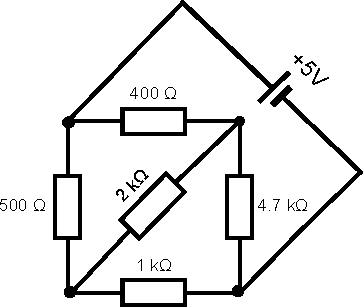
\includegraphics[scale=0.6]{Abbildungen/stromkreis_1.pdf}
		\caption{Beispiel Stromkreis.}
	\end{center}
\end{figure}
\noindent
\paragraph{Die Formulierung in der Elektrostatik} Sei $\Omega$ eine offene Teilmenge des $\mathbb{R}^3$ mit glatten Rand $\partial\Omega$ und $\rho$ die elektrische Ladungsdichte in $\Omega$. Gesucht ist das Potential $\phi:\Omega\rightarrow\mathbb{R}$ sodass:
\begin{align}
\Delta \phi(x) = \rho(x)\text{  falls } x\in \Omega\\
\phi(x) = 0\text{  falls } x\in \partial\Omega
\end{align}
Physikalisch wird $\Omega$ ein Hohlraum in einem guten elektrischen Leiter, wie etwa einem Metall, sein,  da ein Solcher das Potential am Rand des Hohlraumes auf einen konstanten Wert zwingt.\\
\\
Die Elektrostatik lebt im $\mathbb{R}^3$, daher ist die bisher entwickelte Theorie nur in Grenzf\"allen anwendbar. Dieser Spezialfall tritt ein falls $\rho$ und $\Omega$ o.B.d.A entlang der z-Achse konstant sind, daher das Problem effektiv zwei Dimensional wird. F\"ur genau diesen Fall wird eine Theorie der zweidimensionalen Maxwell-Gleichungen im n\"achsten Kapitel entwickelt. 
\begin{proposition}
	Sei $G$ ein  Graph, $r$ eine positive Kantenfunktion und $\Delta_r$ der $r$-gewichtete Laplace Operator, dann gilt:
	\begin{itemize}
		\item Die Form der Matrix $\Delta_r$ is unabh\"angig von der gew\"ahlten Orientierung auf $G$. 
		\item $\Delta_r$ ist symmetrisch.\\
		\item $\Delta_r$ ist positiv semidefinit.\\
		\item Der Kern von $\Delta_r$ ist der Raum der konstanten Eckfunktionen.
	\end{itemize}
\end{proposition}
\begin{proof}
	Seien $p_0$ und $p_1$ Orientierungen auf $G$ und $grad_0$ und $grad_1$ die zugeh\"oringen Gradienten, dann gilt:
	$$grad_0 = D * grad_1$$
	wobei $D$ eine Diagonalmatrix ist, deren Eintr\"age $\pm 1 $ sind. Wegen Satz 2.1 folgt die erste Aussage.\\
	\\
	Die zweite Aussage folgt direkt aus der Definition von $\Delta_r$ und Satz 2.1. Seien hierzu $u$ und $v\in\mathfrak{E}$, dann gilt:
	$$\langle u, \Delta_r(v)\rangle_\mathfrak{E} = \langle \sqrt{r}*\text{grad}(u), \sqrt{r}*\text{grad}(v)\rangle_\mathfrak{K}$$
	Analog zeigt man die dritte Aussage, indem man $u=v$ setzt.
	$$\langle \sqrt{r}*\text{grad}(u), \sqrt{r}*\text{grad}(u)\rangle_\mathfrak{K}\geq 0$$
	Die letzte Aussage: $u\in\text{kern}(\Delta_r)$ gilt genau dann wenn f\"ur jedes $v\in\mathfrak{E}$
	$$\langle v, \Delta_r(u)\rangle_\mathfrak{E}=0$$
	also genau dann wenn
	$$\langle \sqrt{r}*\text{grad}(u), \sqrt{r}*\text{grad}(v)\rangle_\mathfrak{K}=0$$
	Da $r>0$ gilt, ist dies equivalent zu der Aussage $u\in\text{kern}(\text{grad})$. Der Gradient ist genau dann Null wenn $u$ konstant ist, da unser Graph zusammenh\"angend ist.
\end{proof}
\noindent
In der kontinuierlichen Theorie des Poissonproblems sind Sobolevr\"aume und die Poincare Ungleichung von zentraler Bedeutung. Ein Analogon gibt es nat\"urlich auch in der diskreten oder graphischen Theorie.
\begin{proposition}[Poincare Ungleichung]
	Sei $G$ ein Graph, $\partial$ eine Teilmenge der Ecken, $r>0$ eine Kantenfunktion und $u\in\mathfrak{E}$, sodass $u|_\partial=0$ dann gilt:
	$$\langle u, u\rangle_{\mathfrak{E}}\leq \frac{|V|}{\min_{e\in E}r(e)} \langle u, \Delta_r(u)\rangle_{\mathfrak{E}}$$
\end{proposition}
\begin{proof}
	Sei $x\in\partial^c$ and $(x_i)_{i=1}^n$ ein Pfad von $\partial$ nach $x$, dann gilt f\"ur die Pfadsumme:
	$$u(x)^2 = (\sum_{i=1}^{n-1} \sigma_i *\text{grad}(u)(e_i))^2 \leq $$
	$$(\max_{e\in E}\frac{\sum_{s=1}^{n-1}\sqrt{r}(e_s)}{\sqrt{r(e)}})^2*(\sum_{i=1}^{n-1} \sigma_i *\frac{\sqrt{r(e_i)}}{\sum_{s=1}^{n-1}\sqrt{r}(e_s)}\text{grad}(u)(e_i))^2$$
	Wende die Jensen Ungleichung an und fasse zusammen:
	$$u(x)^2\leq (\max_{e\in E}\frac{\sum_{s=1}^{n-1}\sqrt{r}(e_s)}{\sqrt{r(e)}})^2*\sum_{i=1}^{n-1}(\frac{\sqrt{r(e_i)}}{\sum_{s=1}^{n-1}\sqrt{r}(e_s)}\text{grad}(u)(e_i))^2=$$
	$$(\max_{e\in E}\frac{1}{r(e)})*\sum_{i=1}^{n-1} (\sqrt{r}\text{grad}(u)(e_i))^2\leq(\max_{e\in E}\frac{1}{r(e)})*\sum_{k\in E} (\sqrt{r(k)}\text{grad}(u)(k))^2=$$
	$$(\max_{e\in E}\frac{1}{r(e)})*\langle \sqrt{r}\text{grad}(u), \sqrt{r}\text{grad}(u)\rangle_{\mathfrak{K}}=(\max_{e\in E}\frac{1}{r(e)})*\langle u, \Delta_r(u)\rangle_{\mathfrak{E}}$$
	Summieren wir nun \"uber $V$:
	$$\langle u, u\rangle_{\mathfrak{E}}\leq \frac{|V|}{\min_{e\in E}r(e)} \langle u, \Delta_r(u)\rangle_{\mathfrak{E}}$$
\end{proof}
\noindent
Es wurde nun genug Vorarbeit geleistet um das zentrale Existenz Theorem dieses Kapitels zu beweisen.
\begin{theorem}
	Sei $G$ ein Graph, $r$ eine Kantenfunktion, $\partial$ eine Teilmenge der Ecken und $f$ sowie $g$ Eckfunktionen, dann ist das Poissonproblem eindeutig l\"osbar falls $\partial$ nicht leer ist. Wenn $\partial$ jedoch leer ist gibt es nur eine L\"osung wenn $f$ im orthogonalen Komplement der konstanten Funktionen liegt.
\end{theorem}
\begin{proof}
	Falls $\partial$ leer ist, folgt da der Kern von $\Delta_r$ durch die konstanten Funktionen gebildet wird und weil die Abbildung symmetrisch ist, dass der Bildraum das orthogonale Komplement der konstanten Funktionen ist.\\
	\\
	Falls aber $\partial$ nicht leer ist, aber $\partial\neq V$ ist, sollen gilt:\\
	Sei $A$ die Untermatrix die man durch streichen der zu $\partial$ geh\"orenden Zeilen und Spalten erh\"alt.\\
	\\
	Zwei alternative Wege die Trivialit\"at des Kernes von $A$ zu zeigen:\\
	\\
	\textbf{1. Alternative:} Die Poincare Ungleichung zeigt bereits, dass der Kern trivial sein muss.\\
	\\
	\textbf{2. Alternative:}  Sei $x$ ein Element von $\text{kern}(A)$, daher $A(x)=0$. Wir k\"onnen ein Element $\hat{x}$ von $\mathfrak{E}$ konstruieren, sodass $\hat{x}$ an den Ecken die zu $\partial$ geh\"oren Null gesetzt wird und sonst den Wert annimmt den $x$ an der entsprechenden Ecke hat. Es gilt dann:
	$$\Delta_r(\hat{x})|_{E-\partial} = 0$$
	und somit
	$$\langle \sqrt{r}*\text{grad}(\hat{x}),  \sqrt{r}*\text{grad}(\hat{x})\rangle_{\mathfrak{K}} = \langle \hat{x}, \Delta_r(\hat{x})\rangle_{\mathfrak{E}} = 0$$
	Damit muss aber $\hat{x}$ zum Kern von $\Delta_r$ geh\"oren, also eine konstante Funktion sein. Die einzige M\"oglichkeit wie $\hat{x}$ eine konstante Funktion ist, ist wenn es identisch Null ist. Es wurde somit gezeigt, dass der Kern von $A$ trivial ist und somit $A$ invertierbar ist.\\
	\\
	Das Setzen der Randbedingung entspricht aber genau dem Streichen dieser Zeilen sowie Spalten und der Konstruktion einer zugeh\"origen im Allgemeinen von Null verschiedenen Inhomogenit\"at.\\
	\\
	Der Fall $\partial=V$ ist trivialerweise erf\"ullt.
\end{proof}
\noindent
Wandeln wir zur Untermauerung der theoretischen Arbeit an einem Beispiel den elektrischen Stromkreis in Abbildung 3.1 in einen Graphen in dem bisher entwickelten Formalismus um.
\begin{figure}[H]
	\begin{center}
		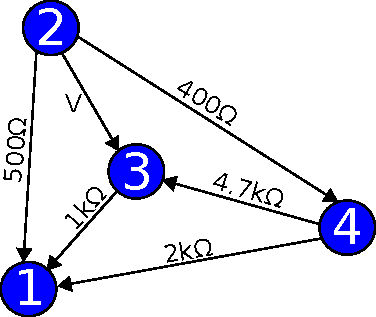
\includegraphics[scale=0.6]{Abbildungen/elektro.pdf}
		\caption{Beispiel Stromkreis (Graph).}
	\end{center}
\end{figure}
\noindent
An den elektrischen Widerst\"anden jeder Kante k\"onnen wir in Abbildung 3.2 die Korrespondenz zu Abbildung 3.1 erkennen. Die Kehrwerte der Widerst\"ande entsprechen der Kantenfunktion $r$ und $\partial=\{2, 3\}$, $g(2)=5$, $g(3)=0$ und $f\equiv 0$. Das $V$ steht f\"ur die Spannungsquelle beziehungsweise die Randbedingung.\\
\begin{center}
$
\Delta_r  = \text{grad}^T * r * \text{grad} = 
\begin{pmatrix}
1 & -1 & 0 & 0\\
1 & 0 & -1 & 0\\
1 & 0 & 0 & -1\\
0 & -1 & 1 & 0\\
0 & 0 & 1 & -1\\
0 & -1 & 0& 1\\
\end{pmatrix}^T
\begin{pmatrix}
\frac{1}{500}& 0 &0& 0& 0&0\\
0& \frac{1}{1000} & 0 & 0 &0&0\\
0 & 0 & \frac{1}{2000} & 0 &0&0\\
0 & 0 & 0 & V & 0&0\\
0 & 0 & 0 & 0 & \frac{1}{4700}&0\\
0 & 0 & 0& 0 & 0 &\frac{1}{400}\\
\end{pmatrix}
\begin{pmatrix}
1 & -1 & 0 & 0\\
1 & 0 & -1 & 0\\
1 & 0 & 0 & -1\\
0 & -1 & 1 & 0\\
0 & 0 & 1 & -1\\
0 & -1 & 0& 1\\
\end{pmatrix}=
\begin{pmatrix}
	\frac{1}{500} + \frac{1}{1000} + \frac{1}{2000}& -\frac{1}{500}  & -\frac{1}{1000} & -\frac{1}{2000}\\
	-\frac{1}{500}  & \frac{1}{500} + V + \frac{1}{400} & -V & -\frac{1}{400}\\
	-\frac{1}{1000} & -V& \frac{1}{1000} + V + \frac{1}{4700} & -\frac{1}{4700} \\
	-\frac{1}{2000} & -\frac{1}{400}&-\frac{1}{4700}  & \frac{1}{400} + \frac{1}{4700} + \frac{1}{2000}
\end{pmatrix}
$
\end{center}
Anschlie\ss{}end wendet man die Randbedingung an, daher man setzt die zweite Komponente des gesuchten Vektors $5$ und die Dritte Komponente $0$, dies entspricht dem streichen der mit $V$ markierten Ecken und bilden der passenden Inhomogenit\"at.
\begin{center}
	$
	\begin{pmatrix}[cc|c]
	\frac{1}{500} + \frac{1}{1000} + \frac{1}{2000} & -\frac{1}{2000} & \frac{5}{500}\\
	-\frac{1}{2000}& \frac{1}{400} + \frac{1}{4700} + \frac{1}{2000} & \frac{5}{400}
	\end{pmatrix}
	$
\end{center}
Dies entspricht genau der Matrixgleichung, die man mit den gebr\"auchlichen Methoden in der Physik zu diesem Problem erh\"alt.\\
\\
Die L\"osung des Poissonproblems erm\"oglicht es uns ein weiteres Analogon zu einem Theorem der klassischen Vektoranalysis zu formulieren.
\begin{corollary}[Helmoltz Zerlegung]
	Sei $G$ ein planarer Graph mit Orientierung dann gilt:
	$$\mathfrak{K}(G) = im(\text{grad}) \bigoplus im(\text{grad}_D)$$
\end{corollary}
\begin{proof}
	Eine Anwendung des de'Rham Komplexes und etwas elementare lineare Algebra liefert:
	$$\mathfrak{K}(G) = \text{kern}(\text{div}_D)\bigoplus\text{kern}(\text{div}_D)^\perp = \text{im}(\text{grad})\bigoplus\text{kern}(\text{div}_D)^\perp$$	
	Die Abbildung $\text{div}_D$ ist ein Isomorphismus zwischen $\text{kern}(\text{div}_D)^\perp$ und $\text{im}(\text{div}_D)$. Wir wissen auch bereits wegen des Theorems 3.2 dass der Laplace Operator des dualen Graphen $\Delta_D = \text{div}_D\circ\text{grad}_D$ ein Isomorphismus zwischen $\mathfrak{F}(G)$ und $\text{im}(\text{div}_D)$. In Kombination zeigt dies, dass $\text{grad}_D$ ein Isomorphismus zwischen $\mathfrak{F}(G)$ und  $\text{kern}(\text{div}_D)^\perp$ ist.
\end{proof}
\chapter{Die Maxwell-Gleichungen}
Die Elektrodynamik beschreibt elektromagnetische Ph\"anomene als durch Felder vermittelte Wechselwirkung von Materie. Diese Felder gehorchen vier Gleichungen, Maxwell-Gleichungen, die im neunzehnten Jahrhundert durch den Schotten James Clerk Maxwell formuliert wurden. Diese partiellen Differentialgleichungen beschreiben wie sich elektromagnetische Felder in Abh\"angigkeit eines Materiestrom zeitlich entwickeln. Die Diskretisierung jener Differentialgleichungen  f\"uhrt im zweidimensionalen Fall zu einer Variante der Maxwell-Gleichungen f\"ur planare Graphen. 
\begin{definition}
	Sei $G$ ein planarer Graph, $r>0$, $\epsilon>0$, $e_0$ Kantenfunktionen, $j\in C^1(\mathbb{R}, \mathfrak{K})$ eine Kurve, $\mu>0$ und $b_0$ Fl\"achenfunktionen und $q_0$ eine Eckfunktion, dann nennt man eine Kurve $e\in C^1(\mathbb{R}, \mathfrak{K})$, eine Kurve $b\in C^1(\mathbb{R}, \mathfrak{F})$  und eine Kurve $e\in C^1(\mathbb{R}, \mathfrak{E})$, sodass f\"ur alle $t\in\mathbb{R}$ gilt:
	\begin{align}
		\text{div}(r * \epsilon * e(t)) = q(t)\\
		\text{div}_D(r^{-1} * e(t)) = -b^\prime(t)\\
		-r^{-1} * \text{grad}_D(b(t) / \mu) = \epsilon * e^\prime(t) + j(t)
	\end{align} 
	und die Anfangsbedingungen
\begin{align}
	e(0) = e_0\\
	b(0) = b_0\\
	q(0) = q_0
\end{align}
erf\"ullt sind, eine L\"osung der Maxwell-Gleichungen.
\end{definition}
\begin{remark}
	(4.1) nennt man das Gau\ss{}sche Gesetz und beschreibt wie das elektrische Feld $e$ mit seinen Quellen den elektrischen Ladungen zusammenh\"angt. Betrachtet man es von der Perspektive eines Flu\ss{}es ist die elektrische Ladung der Nettoflu\ss{} aus der Ecke.\\
	\\
	(4.2) nennt man das Faradaysche Gesetz und es beschreibt die zeitliche \"Anderung des magnetischen Feldes $b$ in Abh\"angigkeit des elektrischen Feldes. Die Kantenfunktion $r$ ist die L\"ange der Kante. $\epsilon$ und $\mu$ sind der elektrische und der magnetische Leitwert, respektive. Diese beiden Funktionen geben an wie gut die Kanten das Feld durchlassen.\\
	\\
	(4.3) nennt man das Amperesche Gesetz und beschreibt analog zum Faradayschen Gesetz wie die zeitliche \"Anderung des elektrischen Feldes vom magnetischen Feld, aber auch vom elektrischen Strom $j$ abh\"angig ist. Wenn wir das Ohmsche Gesetz $j(t) = \sigma e(t)$ annehmen, verh\"alt sich der elektrische Strom hier wie ein Reibungsterm. Wir werden sehen, dass dies tats\"achlich f\"ur Energieverlust ins W\"armebad verantwortlich ist.
\end{remark}
\noindent
Aus den Maxwell-Gleichungen ergeben sich die Erhaltungsgr\"o\ss{}en elektrische Ladung und Energie. Die Energie teilt sich in magnetische und elektrische Energie, die \"uber die Zeit innernander umgewandlet werden.
\begin{proposition}\textbf{Energieerhaltung}
	Sei $G$ ein planarer Graph, $r>0$, $\epsilon>0$, $e_0$ Kantenfunktionen, $\mu>0$ und $b_0$ Fl\"achenfunktionen, $q_0$ eine Eckfunktion und  $e:\mathbb{R}\rightarrow\mathfrak{K}(G)$ das elektrische Feld und $b:\mathbb{R}\rightarrow\mathfrak{F}(G)$ das magnetische Feld L\"osungen der Maxwell-Gleichungen, dann nennt man 
	\begin{equation}
	E = \frac{1}{2}(\sum_{a\in f} b(a)^2 /\mu(a) + \sum_{k\in E} \epsilon(k) * e(k)^2)
	\end{equation}
	die \textbf{Energie} und solange der elektrische Strom $j\equiv 0$ gilt, bleibt die Energie unver\"andert. 
\end{proposition}
\begin{proof}
	Sei $e$ und $b$ wie in der Voraussetzung des Satzes dann gilt f\"ur die Ableitung der magnetischen Energie:
	$$(\sum_{a\in f} b(a)^2 /\mu(a))^\prime = \sum_{a\in f} 2 * b(a) * b(a)^\prime /\mu(a) = -\sum_{a\in f} 2 * b(a) * \text{div}_D(r^{-1} * e)(a) /\mu(a)=$$
	$$-2 * \langle b /\mu, \text{div}_D(r^{-1} * e\rangle_{\mathfrak{F}}$$
	und f\"ur die Ableitung der elektrischen Energie:
	$$(\sum_{k\in E} \epsilon(k) * e(k)^2)^\prime = \sum_{k\in E} 2 * \epsilon(k) * e(k) * e(k)^\prime = $$
	$$-\sum_{k\in E} 2 * e(k) * (r^{-1} * \text{grad}_D(b /\mu) + j) (k)=-2 * \langle e, (r^{-1} * \text{grad}_D(b /\mu) + j) \rangle_{\mathfrak{K}}=$$
	$$2 * (\langle \text{div}_D(r^{-1} * e), b /\mu\rangle_{\mathfrak{F}} - \langle e, j\rangle_{\mathfrak{K}})$$
	Fassen wir zusammen:
	$$E^\prime = -\langle e, j\rangle_{\mathfrak{K}}$$
\end{proof}
\begin{proposition}\textbf{Kontinuit\"atsgesetz}
	Sei $G$ ein planarer Graph, $r>0$, $\epsilon>0$, $e_0$ Kantenfunktionen, $\mu>0$ und $b_0$ Fl\"achenfunktionen, $q_0$ eine Eckfunktion und  $e:\mathbb{R}\rightarrow\mathfrak{K}(G)$ das elektrische Feld und $b:\mathbb{R}\rightarrow\mathfrak{F}(G)$ das magnetische Feld L\"osungen der Maxwell-Gleichungen, dann gilt das Kontinuit\"atsgesetz:
	$$q^\prime = - \text{div}(r*j)$$
	Dies zeigt, dass die Gesamtladung erhalten bleibt.
\end{proposition}
\begin{proof}
	Dividiere (4.3) in Definition 4.1 durch $\epsilon$ und dann wende $\text{div}(r * \epsilon * .)$ auf (4.3) an:
	$$\text{div}(r * \epsilon * (-\epsilon^{-1} * r^{-1} * \text{grad}_D(b(t) / \mu))) = \text{div}(r * \epsilon * (e^\prime + j/\epsilon))$$
	$$0 = \text{div}(r * \epsilon * e)^\prime + \text{div}(r * j))$$
	$$0 = q^\prime + \text{div}(r * j)$$
	Summieren wir nun die obige Gleichung \"uber alle Ecken, dann heben sich die Beitr\"age der Kanten in $\text{div}(r*j)$ gegenseitig auf, da jede Kante einmal in dem $\text{div}$-Term der Ecke von der er wegzeigt und einmal im Term der Ecke auf die er zeigt vorkommt. Folglich gilt:
	$$\sum_{v\in V}q^\prime=0$$
\end{proof}
\noindent
Die Maxwell-Gleichungen sind ein System gew\"ohnlicher linearer Differentialgleichungen und als solches gibt es keine Probleme wegen Existenz und Eindeutigkeit f\"ur jeden Zeitpunkt. Dies l\"asst sich in jedem guten Buch \"uber gew\"ohnliche Differentialgleichungen nachlesen.
\begin{theorem}
	Die Maxwellgleichungen sind eindeutig l\"osbar, solange die Anfangsbedingung (4.1) erf\"ullt ist.
\end{theorem}
\begin{proof}
\end{proof}
\chapter{Potentialformulierung der Maxwellgleichungen}
Analog zum kontinuierlichen Fall lassen sich die Maxwellgleichungen auf planaren Graphen \"uber Potentiale ausdr\"ucken. 
\begin{definition}
Sei $G$ ein planarer Graph mit Orientierung und $r>0$ eine Kantenfunktion auf $G$, dann definieren wir eine Transformation $T$,
die Kurven $(\phi, a)\in C^1(\mathbb{R},\mathfrak{E})\times C^1(\mathbb{R},\mathfrak{K})$ in Felder $(e, b)\in C^1(\mathbb{R},\mathfrak{K})\times C^1(\mathbb{R},\mathfrak{F})$ \"uberf\"uhrt, durch
	\begin{align}
		\left(
		\begin{array}{c}
		b(t)\\
		e(t)
		\end{array}
		\right)=
		T(\left(
		\begin{array}{c}
		\phi(t)\\
		a(t)
		\end{array}
		\right))=
		\left(
		\begin{array}{c}
		\text{div}_D(r^{-1}a(t))\\
		-a^\prime(t) - r\text{grad}(\phi(t))
		\end{array}
		\right)
	\end{align}
 f\"ur alle $t\in\mathbb{R}$. Die Kurven $\phi$ und $a$ nennt man Potentiale, ersteres ist das Skalarpotential und letzteres das Vektorpotential.
\end{definition}
\noindent
Es ist hierbei zu bedenken, dass $\text{div}_D$ nicht surjektiv ist, sondern nur Fl\"achen-funktionen darstellen kann, die orthogonal zu den konstanten Funktionen sind. Dies scheint auf den ersten Blick eine Einschr\"ankung zu sein, aber eine kurze Betrachtung der Maxwellgleichungen zeigt uns, dass der konstante Anteil des Magnetfeldes keine Auswirkung auf das elektrische Feld hat, solange $\mu$ konstant ist. Viel wichtiger noch findet die einzige \"Anderung des Magnetfeldes, die unter G\"ultigkeit der Maxwellgleichungen passieren darf im orthogonalen Komplement der konstanten Fl\"achenfunktionen statt.\\
Wir fordern nun zus\"atzlich zu den Maxwellgleichungen, dass das Magnetfeld $b$
f\"ur jeden Zeitpunkt $t\in\mathbb{R}$ orthogonal zu den konstanten Fl\"achenfunktionen ist: 
$$b(t)\in \mathbb{R}^\perp$$
Wenn wir planare Graphen als Polyeder auffassen, ist dies einfach das im dreidimensionalen g\"ultige Gau\ss{}sche Gesetz f\"ur Magnetfelder.\\
\\
Die Wahl der Potential Definition kam nicht von ungef\"ahr, sondern aus der Theorie im Kontinuum. 
Die Definition des Magnetfeldes in (5.1) abgeleitet ergibt durch Einsetzen der Definition des elektrischen Feldes sofort das Faradaysche Gesetz. 
Nachdem das Gaußsche Gesetz als Definition der elektrischen Ladung gesehen werden kann, reduzieren sich die Maxwellgleichungen in Potentialformulierung auf das Amperesche Gesetz: 
\begin{equation}
r^{-1}\text{grad}_D(\text{div}_D(r^{-1}a(t)) / \mu) = \epsilon * (a^{\prime\prime} + r\text{grad}(\phi^\prime)) - j(t)
\end{equation}
Der Vorteil der Potentialdarstellung liegt zum Einen in der Vereinfachung des Gleichungssystems und zum Anderen in der gr\"o\ss{}eren Flexibilit\"at.\\
\\
Es ist leicht zu sehen, dass die Operation aus Definition 5.1, die Potentiale in Felder umwandelt nicht injektiv ist.\\
\\
Die Charakterisierung des Kerns dieser linearen Operation f\"uhrt uns nun zu den so genannten Eichtransformationen.
\begin{definition}
	Seien $\phi$ und $a$ Potentiale wie in Definition 5.1, und $\xi\in C^1(\mathbb{R}, \mathfrak{E})$, dann nennt man die Transformation $T$ definiert durch
\begin{equation}
\gamma_\xi(\left(
\begin{array}{c}\phi\\
a
\end{array}\right))=
\left(
\begin{array}{c}\phi - \xi^\prime\\
a + r\text{grad}(\xi) 
\end{array}\right)
\end{equation}
	die zu $\xi$ geh\"orende \textbf{Eichtransformation}.
\end{definition}
\noindent
Die Potentiale werden immer genau bis auf eine Eichtransformation eindeutig durch die Felder bestimmt.
\begin{proposition}
	Sei $T$ die lineare Operation aus Definition 5.1, die Potentiale $(\phi, a)\in C^1(\mathbb{R},\mathfrak{E})\times C^1(\mathbb{R},\mathfrak{K})$ in Felder $(e, b)\in C^1(\mathbb{R},\mathfrak{K})\times C^1(\mathbb{R},\mathfrak{F})$ \"uberf\"uhrt, dann gilt:
	\begin{equation}
	\text{kern}(T)=\{\left(
	\begin{array}{c}-\xi^\prime\\
	r\text{grad}(\xi)
	\end{array}\right)| \xi\in C^1(\mathbb{R},\mathfrak{E})\}
	\end{equation}
\end{proposition}
\begin{proof}
Wir starten mit der Inklusion $(\supset)$\\
Sei $(\phi, a)\in \text{kern}(T)$, dann gilt f\"ur alle $t\in\mathbb{R}$
\begin{equation*}
	0 = \text{div}_D(r^{-1}a(t))
\end{equation*} 
Wir wissen wegen dem de'Rham Komplex Theorem, und weil $r>0$ ist, dass es eine  $\chi:\text{im}(\text{grad})\mapsto \mathbb{R}^\perp$ gibt, sodass gilt:
\begin{equation*}
	x = \text{grad}(\chi(x)) \text{ f\"ur  alle }x\in\mathfrak{K}(G)
\end{equation*}
Daher k\"onnen wir f\"ur alle $t\in\mathbb{R}$ definieren 
\begin{equation*}
\xi(t) = \chi(r^{-1}a(t))
\end{equation*} sodass gilt
\begin{equation*}
	a=r\text{grad}(\xi)
\end{equation*} und $\xi\in C^1(\mathbb{R},\mathfrak{E})$.\\
Wir setzen den so gewonnenen Ausdruck f\"ur $a$ nun ein in
\begin{equation*}
	0=-a^\prime(t) - r\text{grad}(\phi(t))
\end{equation*} 
und erhalten f\"ur alle $t\in\mathbb{R}$
\begin{equation*}
0=\text{grad}(\xi^\prime(t)+\phi(t))
\end{equation*} 
Somit gilt die Gleichheit modulo einer Konstante $c$
\begin{equation*}
\phi(t)=-\xi^\prime(t) +c
\end{equation*}
Die Konstante $c$ kann man weil sie im Kern des Gradienten liegt in $\xi$ einziehen.
\begin{equation*}
	\xi(t) = \chi(r^{-1}a(t)) -c*t
\end{equation*}
\noindent
Die andere Inklusion $(\subset)$ wird gezeigt indem der Ausdruck in der Mengendefinition (5.4) in $T$ eingesetzt wird.
\end{proof}
\noindent
Hiermit wurden die wichtigsten Aspekte der Potentialdarstellung vorgestellt. Dies ist eine Grundvoraussetzung f\"ur die Quantisierung der Maxwellgleichungen.\\
\\
Zum Abschlu\ss{} dieses Kapitels konstruieren wir eine L\"osung der Maxwellgleichungen in Potentialdarstellung (5.2) im stromlosen Fall $j\equiv 0$.\\
\\
Wegen der Eichinvarianz von (5.2) gibt es immer eine L\"osung mit $\phi\equiv0$, wodurch wir ohne Beschr\"ankung der Allgemeinheit $\phi$ aus (5.2) eliminieren k\"onnen.
\begin{lemma}
	Sei $L$ eine positiv semidefinite lineare Abbildung in $V=\mathbb{R}^n$ ($n\geq 1 $), $u_0, v_0 \in V$ und $u\in C^2(\mathbb{R}, V)$, dann ist die L\"osung des Anfangswertproblems
	\begin{align}
		u^{\prime \prime} + L&u = 0\\
		u(0) &= u_0\\
		u^\prime(0)&=v_0
	\end{align}
	gegeben durch
	\begin{equation}
		u(t) = U^\dagger (\cos(Rt) + 1_{\{0\}}(R))Uu_0 +U^\dagger (\sin(Rt) + 1_{\{0\}}(R)t)Uv_0
	\end{equation}
	Wobei $U$ eine orthogonale, R eine Diagonalmatrix in $V$ ist und $L=U^\dagger R^2 U$ gilt.
\end{lemma}
\begin{proof}
	Nach dem Spektralsatz endlichdimensionaler reeler Vektorr\"aume gibt es eine Zerlegung der positiv semidefiniten Matrix $L$ der Form.
	\begin{equation*}
		L=U^\dagger R^2 U
	\end{equation*}
	Wobei $R\geq 0$ und $U$ eine orthogonale Matrix ist.
	\\
	\\
	Als n\"achstes formen wir (5.2) um
	\begin{align*}
		U(u^{\prime \prime} + Lu )&= 0\\
		(Uu)^{\prime \prime} + ULu &= 0\\
		(Uu)^{\prime \prime} + ULU^\dagger Uu &= 0
	\end{align*}
 und setzen $v=Uu$
 \begin{equation}
	v^{\prime \prime} + R^2v=0
 \end{equation}
Die allgemeine L\"osung von (5.9) erhalten wir wenn f\"ur jede Komponente $n>1$
\begin{equation*}
	v_n(t) = 
	\begin{cases} 
		v_n(0)\cos(R_nt) + v_n^\prime(0)\sin(R_nt) & R_n > 0 \\
		v_n(0) + v_n^\prime(0)t & R_n=0 
	\end{cases}	
\end{equation*} 
 f\"ur $t\in\mathbb{R}$. In Matrixform umgeschrieben erhalten wir (5.8).
\end{proof}
\begin{proposition}
Sei $G$ ein planarer Graph mit Orientierung, $r>0$, $a_0$, $e_0$ Kantenfunktionen, $\mu>0$ eine Fl\"achenfunktion auf $G$ und $\epsilon>0$, dann gibt es eine Kurve $a\in C^2(\mathbb{R},\mathfrak{K})$, sodass f\"ur alle $t\in\mathbb{R}$ gilt
\begin{equation}
	a^{\prime\prime}(t)-r^{-1}\text{grad}_D(\text{div}_D(r^{-1}a(t)) / \mu) / \epsilon = 0
\end{equation}
und die Anfangsbedingung
\begin{align}
	a(0)&= a_0\\
	a^\prime(0) &= e_0
\end{align}
erf\"ullt ist.
\end{proposition}
\begin{proof}
Es verbleibt zu zeigen, dass die lineare Abbildung $L$ definiert f\"ur $u\in \mathfrak{K}$ durch 
\begin{equation*}
	L(u) = -r^{-1}\text{grad}_D(\text{div}_D(r^{-1}u) / \mu) / \epsilon
\end{equation*}
positiv semidefinit ist:
\begin{align*}
	\langle u, L(u)\rangle_{\mathfrak{K}} = 
	&\langle u, -r^{-1}\text{grad}_D(\text{div}_D(r^{-1}u) / \mu) / \epsilon\rangle_{\mathfrak{K}} =\\ 
	&\langle r^{-1}u, -\text{grad}_D(\text{div}_D(r^{-1}u) / \mu) \rangle_{\mathfrak{K}}/ \epsilon=\\
	&\langle \text{div}_D(r^{-1}u), \text{div}_D(r^{-1}u) / \mu\rangle_{\mathfrak{F}}/ \epsilon\geq 0
\end{align*}
\end{proof}

\iffalse
Schlie\ss{}en wir dieses Kapitel ab indem wir f\"ur den stromlosen Fall $j\equiv0$ eine L\"osung zu (5.2) konstruieren .
Wegen der Eichinvarianz von (5.2) gibt es immer eine L\"osung mit $\phi\equiv0$, wodurch sich (5.2) auf
\begin{equation}
	a^{\prime\prime}-r^{-1}\text{grad}_D(\text{div}_D(r^{-1}a(t)) / \mu) / \epsilon=0
\end{equation}
reduziert.

Wir definieren die positiv semidefinite Matrix\\ $Q=-r^{-1}\text{grad}_D(\text{div}_D(r^{-1}a(t)) / \mu) / \epsilon$ und formulieren (5.5) kompakter als
\begin{equation}
	a^{\prime\prime}+Qa(t)=0
\end{equation}
Hierbei ist $Q$ ein positiv semidefiniter Operator.
Als n\"achstes transformieren wir die lineare Differentialgleichung zweiter Ordnung in eine equivalent erster Ordnung.
\fi
\noindent
Falls $\epsilon>0$ nicht konstant ist, k\"onnen wir auch eine L\"osung konstruieren. Hierzu transformieren wir zun\"achst (5.5) in eine Differentialgleichung erster Ordnung.
\begin{equation}
		\begin{pmatrix}
		a  \\ u 
	\end{pmatrix}^\prime=
	\begin{pmatrix}
		0 & \mathbb{I} \\ 
		L & 0
	\end{pmatrix}
	\begin{pmatrix}
	a  \\ u 
	\end{pmatrix}
\end{equation}
Die allgemeine L\"osung dieser Gleichung zu Anfangsbedingungen $a(0)=a_0\in\mathfrak{K}$ und $u(0)=a^\prime(0)=u_0\in\mathfrak{K}$ lautet f\"ur jedes $t\in\mathbb{R}$
\begin{equation}
\begin{pmatrix}
	a  \\ u 
\end{pmatrix}(t)=
e^{	\begin{pmatrix}
		0 & \mathbb{I} \\ 
		L & 0
\end{pmatrix}t}
	\begin{pmatrix}
	a_0  \\ u_0 
\end{pmatrix}=
\sum_{n=0}^\infty \frac{\begin{pmatrix}
		0 & \mathbb{I} \\ 
		L & 0
	\end{pmatrix}^nt^n}{n!}\begin{pmatrix}
a_0  \\ u_0 
\end{pmatrix}
\end{equation}
Das Matrixexponential kann als Potenzreihe oder mit Hilfe der reelen Jordanschen Normalform der Matrix $M=\begin{pmatrix}
	0 & \mathbb{I} \\ 
	L & 0
\end{pmatrix}$ wie im Hilfssatz 5.3 konstruiert werden.
\iffalse
\\
\\
\textbf{Zur Konstruktion der Jordanschen Normalform:}\\
Sei $\omega\in\sigma(L)$ ein Eigenwert von $L$ mit Eigenvektor $v_\omega$. 
\\
Falls $\omega\neq 0$, dann k\"onnen wir zwei Eigenvektoren $u_{\pm\sqrt{\omega}}=\begin{pmatrix}
	v_\omega \\ \pm\sqrt{\omega}v_\omega
\end{pmatrix}$ zu den Eigenwerten $\pm\sqrt{\omega}$   von $M$ konstruieren. 
\\
\\
Falls $\omega=0$ k\"onnen wir f\"ur jeden zugeh\"origen Eigenvektor $v$ nur einen einzigen Eigenvektor $u=\begin{pmatrix}
v \\ 0
\end{pmatrix}$ von $M$ konstruieren. Entsprechend wird  zu jedem Eigenvektor $v$ auch ein Hauptvektor $u_h=\begin{pmatrix}
u_h^1  \\ u_h^2 
\end{pmatrix}$ konstruiert, sodass
\begin{equation*}
	M^2u_h = \begin{pmatrix}
		L & 0 \\ 
		0 & L
	\end{pmatrix}\begin{pmatrix}
	u_h^1  \\ u_h^2 
\end{pmatrix}
\end{equation*}
\fi
\chapter{Kanonische Quantisierung des elektromagnetischen Feldes}
Anfang des zwanzigsten Jahrhunderts wurde zur Erkl\"arung einer Reihe von Ph\"anomenen, die innerhalb der damals etablierten/klassischen physikalischen Theorien nicht erkl\"arbar waren, die Quantentheorie entwickelt.
Die Objekte der klassischen Theorien sind Kurven, Kr\"afte und Felder und in der Quantenmechanik sind es Zustandsvektoren, Operatoren und Distributionen. Die messbaren Gr\"o\ss{}en bleiben dieselben, allerdings werden die mathematischen Objekte, die ihr Verhalten beschreiben etwas komplizierter.\\
\\
Wir wollen nun den klassischen Weg der Quantisierung einer physikalischen Theorie am Beispiel der Maxwellgleichungen auf planaren Graphen erkunden.\\
\\
Der Ausgangspunkt dieser so genannten kanonischen Quantisierung ist die Lagrangefunktion der Theorie.
\begin{theorem}
Sei $G$ ein planarer Graph, $r>0$, $\epsilon>0$,  Kantenfunktionen, $q\in C^1(\mathbb{R}, \mathfrak{E})$, $j\in C^1(\mathbb{R}, \mathfrak{K})$, sodass gilt
\begin{equation}
	q^\prime = - \text{div}(r*j)
\end{equation}
Sei weiters $\mu>0$ eine Fl\"achenfunktion dann sind $a$ und $\phi$ L\"osungen der Maxwellgleichung in Potentialform (5.2), genau dann wenn alle Richtungs-ableitungen des Wirkungsfunktionals verschwinden auf dem Raum der $f_1\in C^1(\mathbb{R}, \mathfrak{E})$ und $f_2\in C^1(\mathbb{R}, \mathfrak{K})$ f\"ur die gilt, dass $f_1$ und $\phi$ sowie $f_2$ und $a$ zu den Zeitpunkten $r$ und $s$ \"ubereinstimmen
\begin{equation}
	S(f_1, f_2) = \int_{r}^{s}W(f_1, f_2, f_1^\prime, f_2^\prime)dt
\end{equation}
\noindent
Die Funktion unter dem Integral nennt man die \textbf{Lagrangefunktion} der Maxwellgleichung.
Sie ist dabei gegeben durch:
\begin{align*}
	L(q_1, q_2, v_1, v_2) =&\frac{1}{2}(\langle \epsilon(v_2 + r\text{grad}(q_1)), v_2 + r\text{grad}(q_1)\rangle_\mathfrak{K} -\\& \langle\text{div}_D(r^{-1}q_2), \text{div}_D(r^{-1}q_2)/\mu\rangle_\mathfrak{F}) + \langle q_2, j\rangle_\mathfrak{K} - \langle q_1, q\rangle_\mathfrak{E}
\end{align*}
\end{theorem}
\begin{proof}
Siehe beliebiges Fachbuch zur theoretischen Physik.
\end{proof}
\noindent
Im n\"achsten Schritt wollen wir diese Lagrangefunktion \"uber eine Legendre Transformation in die zugeh\"orende \textbf{Hamiltonfunktion} umgewandelt.
\begin{definition}
	Sei $f:X\mapsto\mathbb{R}$ eine konvexe Funktion auf einem Skalarproduktraum $X$, dann ist die \textbf{Legendretransformation} $f^*$ definiert durch:
	\begin{equation}
		f^*(y) = \sup_{x\in X}(\langle x, y\rangle-f(x))
	\end{equation}
\end{definition}
\noindent
Jedoch wollen wir zun\"achst ein n\"utzliches Resultat zeigen mit dessen Hilfe wir eine wohldefinierte Legendretransformation samt Formel erhalten.
\begin{proposition}
	Sei $f:X\mapsto\mathbb{R}$ eine strikt konvexe stetig differenzierbare Funktion auf einem Skalarproduktraum $X$, sodass die Abbildung $x\mapsto Df(x)$ invertierbar ist, dann ist die Legendretransformation gegeben durch:
	\begin{equation}
		f^*(y) = \langle (Df)^{-1}(y), y\rangle-f((Df)^{-1}(y))
	\end{equation}
\end{proposition}
\begin{proof}
Die Funktion $g_y(x)=\langle x, y\rangle-f(x)$ ist streng konkav und hat daher ein eindeutiges Maximum $x_0\in X$.
\begin{equation*}
	Dg_y(x_0) = y - Df(x_0)=0\Rightarrow x_0 = (Df)^{-1}(y)
\end{equation*}
Eingesetzt in $g_y$ erhalten wir dann
\begin{equation*}
	f^*(y)=g_y(x_0) = \langle (Df)^{-1}(y), y\rangle-f((Df)^{-1}(y))
\end{equation*}
\end{proof}
\noindent
Um diese Darstellung ausnutzen zu k\"onnen m\"ussen wir die Lagrangefunktion strikt konvex machen, indem wenn wir das Skalarpotential $\phi$ aus der Lagrangefunktion entfernen.\\
Dies ist m\"oglich, da es zu jeder Paarung eines Skalarpotentials und eines Vektorpotentials eine Eichtransformation gibt, die diese in ein Paar umwandelt, dessen Skalarpotential gleich Null ist.\\
\\
Die resultierende Lagrangefunktion ist gegeben durch 
\begin{equation}
	L(q, v) =\frac{1}{2}(\langle \epsilon v, v\rangle_\mathfrak{K} - \langle\text{div}_D(r^{-1}q), \text{div}_D(r^{-1}q)/\mu\rangle_\mathfrak{F}) + \langle q, j\rangle_\mathfrak{K}
\end{equation}
\noindent
Das \"ubrige Vektorpotential (hier q) ist immer noch nicht eindeutig bestimmt, und die Eichtransformationen die diese Form der Eichung erhalten sind genau jene, die laut Definition (5.2) zu einem konstanten $\xi$ korrespondieren.\\
\\
Die Hamiltonfunktion erhalten wir durch eine Anwendung der Legendretransformation auf die Lagrangefunktion (6.5) bez\"uglich der Variablen $v$.
\begin{equation}
	H(\pi, q) = \frac{1}{2}\langle \frac{\pi}{\epsilon}, \pi\rangle_{\mathfrak{K}} + \frac{1}{2}\langle \text{div}_D(r^{-1}q), \text{div}_D(r^{-1}q)/\mu\rangle_{\mathfrak{F}} - \langle q, j\rangle_{\mathfrak{K}}
\end{equation}
Wenn wir mit (4.7) der Energieerhaltung, Satz (4.1), vergleichen, erkennen wir, dass, die ersten beiden Terme genau die dort proklamierte Gesamtenergie sind und der \"ubrige Term genauso beschaffen scheint um die zeitliche Ableitung nach Satz 4.1 zu kompensieren. Solange $j$ zeitunabh\"anging ist, und somit auch $H$ nicht explizit von der Zeit abh\"angt, ist dies auch der Fall.\\
\\
Mit Hilfe der Euler-Lagrange-Gleichung k\"onnen wir nun die \textbf{Hamiltonschen Bewegungsgleichungen} herleiten.
\begin{proposition}
Sei $G$ ein planarer Graph, $r>0$, $\epsilon>0$,  Kantenfunktionen, $j\in C^1(\mathbb{R}, \mathfrak{K})$, $\mu>0$ eine Fl\"achenfunktion dann sind $a$ und $\phi$ L\"osungen der Maxwellgleichung in Potentialform (5.2), genau dann wenn die Hamiltonschen Bewegunggleichungen erf\"ullt sind:
\begin{align}
	q^\prime = \frac{\partial H}{\partial \pi}\\
	\pi^\prime = - \frac{\partial H}{\partial q}
\end{align}
\end{proposition}
\begin{proof}
	Siehe beliebiges Fachbuch zur theoretischen Physik.
\end{proof}
\noindent
An diesem Punkt entfernen wir uns von der klassischen Theorie und folgen Heisenberg in die Quantenmechanik. Die Kurven $\pi$ und $q$ aus $C^1(\mathbb{R}, \mathfrak{K})$ sind von nun an Kurven $\hat{\pi}$ und $\hat{q}$ in einem Raum von Operatoren auf einem Hilbertraum.\footnote{Operator auf einem Hilbertraum bedeutet ein dicht definierter linearer Operator.}
\begin{definition}
	Sei $G$ ein planarer Graph und $r>0$ eine Kantenfunktion, dann ist der Hilbertraum unserer Theorie gegeben durch
	\begin{equation}
		\mathfrak{H} = L^2(\mathfrak{K}(G),\mathbb{C};\lambda)
	\end{equation}
	Der Raum der komplexen Funktionen auf $\mathfrak{K}(G)$ deren Quadrate ein endliches Integral bez\"uglich dem Ma\ss{} $\lambda$\footnote{$\lambda$ wird zu einem sp\"ateren Zeitpunkt festgelegt.} hat.\\
	\\
	Das Skalarprodukt von $\xi,\phi\in\mathfrak{H}$ ist dabei definiert durch:
	\begin{equation}
		\langle \phi, \xi\rangle_{\mathfrak{H}} = \int_\mathfrak{K} \overline{\phi}(x)\xi(x)d\lambda(x)
	\end{equation}
\end{definition}
\noindent
\paragraph{Interpretation}
\begin{itemize}
\item Jedes Element $\psi\in\mathfrak{H}$ stellt einen m\"oglichen Zustand des quantisierten elektromagnetischen Feldes dar. 
\item Jeder Messgr\"o\ss{}e $\Omega$ des klassischen elektromagnetischen Feldes entspricht ein korrespondierender Operator $\hat{\Omega}$ auf $\mathfrak{H}$. 
\item Der Ausgang einer Messung der Gr\"o\ss{}e $\Omega$ ist ein zuf\"alliges Element des Spektrums von $\Omega$ und der Mittelwert der Messungen ist gleich $\frac{\langle \psi, \hat{\Omega}\psi\rangle_{\mathfrak{H}}}{\langle \psi, \psi\rangle_{\mathfrak{H}}}$.
\end{itemize}
\noindent
Widmen wir uns nun der Konstruktion der korrespondierenden Operatoren. Nach Heisenberg wird f\"ur jedes Kantenpaar $e,e'\in E$ die kanonische Vertauschungsrelation:
\begin{equation}
	[\hat{q}(e), \hat{\pi}(e')] = i\delta_{e, e'}
\end{equation}
gefordert.\\
\\
Eine m\"ogliche Darstellung dieser Operatoren $\hat{q}(k)$ und $\hat{\pi}(k)$, die (6.10) erf\"ullt ist gegeben durch:
\begin{align}
	\hat{\pi}(k):(q\mapsto\psi(q)) \mapsto (q\mapsto -i\frac{\partial\psi}{\partial q_k}(q))\text{  f\"ur }k\in E\\
	\hat{q}(k):(q\mapsto\psi(q)) \mapsto (q\mapsto q_k\psi(q))\text{  f\"ur }k\in E
\end{align}
\noindent
Hierbei ist $q_k$ der Wert der Kantenfunktion $q$ an der Stelle $k\in E$ und $\frac{\partial}{\partial q_k}$ ist die Ableitung nach demselben Wert. Der Definitionsbereich $D(\hat{\pi}(k))$ und $D(\hat{q}(k))$ f\"ur $k\in E$ wird zu einem sp\"ateren Zeitpunkt festgelegt und bleibt bis dahin eine unbekannte dichte Teilmenge von $\mathfrak{H}(G)$.
\\
\\
Eine kurze Betrachtung der Hamiltonfunktion (6.4) zeigt die \"Aquivalenz dieses Problems zu der Bewegung von $|E|$ Punktma\ss{}en mit Massen $\epsilon(k)$ f\"ur jedes $k\in E$ in einem Potential. 
\begin{definition}
	Sei $G$ ein planarer Graph, $r>0$, $\epsilon>0$, $e_0$ Kantenfunktionen, $\hat{j}$ eine Kurve selbstadjungierter Operatoren auf $\mathfrak{H}(G)$, $\mu>0$ und $b_0$ Fl\"achenfunktionen, dann ist der Hamiltonoperator $\hat{H}:D(\hat{H})\rightarrow \mathfrak{H}(G)$ des elektromagnetischen Feldes gegeben durch:\footnote{$D(\hat{H})$ ist eine dichte Teilmenge von $\mathfrak{H}(G)$ die zu einem sp\"ateren Zeitpunkt festgelegt wird.}
	\begin{equation}
	\hat{H}=-\sum_{k\in E}\frac{1}{2\epsilon(k)}\frac{\partial^2}{\partial q_k^2} + \frac{1}{2}\langle \text{div}_D(r^{-1}q), \text{div}_D(r^{-1}q)/\mu\rangle_{\mathfrak{F}} - \langle q, \hat{j}\rangle_{\mathfrak{K}}
	\end{equation}
	Sei $\psi_0\in D(\hat{H})$ und $\psi\in C^1(\mathbb{R}, D(\hat{H}))$, sodass:
\begin{equation}
\hat{H}\psi(t) = i\psi^\prime(t)
\end{equation}
f\"ur alle $t\in\mathbb{R}$ gilt und die Anfangsbedingung $\psi(0)=\psi_0$ erf\"ullt ist, dann nennt man $\psi$ eine L\"osung der
\textbf{Schr\"odingergleichung} des elektromagnetischen Feldes.
\end{definition}
\noindent
Widmen wir uns nun dem Korrespondenzprinzip zwischen der klassischen und quantenmechanischen Theorie.
Wir werden zeigen, dass die durch die Schr\"odingergleichung vermittelte Dynamik im Mittel mit jener der Maxwellgleichungen \"ubereinstimmt. 
\begin{theorem}[Ehrenfest Theorem]
	Sei $G$ ein planarer Graph, $\epsilon>0$ und $r>0$ Kantenfunktionen, $\mu>0$ eine Fl\"achenfunktion und $\psi: \mathbb{R}\mapsto \mathfrak{H}$ eine L\"osung der Schr\"odingergleichung (6.14) auf $G$, dann gilt:
	\begin{align}
		&\epsilon\langle \psi, \hat{e}\psi\rangle_{\mathfrak{H}}^\prime =  -r^{-1} \text{grad}_D(\langle\psi,\hat{b}\psi\rangle_{\mathfrak{H}}/\mu) -  \langle \psi, \hat{j} \psi\rangle_{\mathfrak{H}}\\
		&\langle \psi, \hat{b}\psi\rangle_{\mathfrak{H}}^\prime = -\text{div}_D(r^{-1}\langle\psi, \hat{e}\psi\rangle_{\mathfrak{H}})
	\end{align}
	wobei der elektrische und magnetische Feldoperator gegeben sind durch:
	\begin{align}
		&\hat{e} = \frac{-\hat{\pi}}{\epsilon}\\
		&\hat{b} = \text{div}_D(r^{-1}\hat{q})
	\end{align}
\end{theorem}
\begin{proof}
Wir starten mit der linken Seite von (6.15), wenden die Produktregel der Differentiation an und formen um:
\begin{align*}
	&\epsilon\langle \psi, \hat{e}\psi\rangle_{\mathfrak{H}}^\prime = -\langle \psi, \hat{\pi}\psi\rangle_{\mathfrak{H}}^\prime=\\
	&-(\langle \psi^\prime, \hat{\pi}\psi\rangle_{\mathfrak{H}}+\langle \psi, \hat{\pi}\psi^\prime\rangle_{\mathfrak{H}})=\\
	&\langle i\hat{H}\psi, \hat{\pi}\psi\rangle_{\mathfrak{H}}+\langle \psi, \hat{\pi}i\hat{H}\psi\rangle_{\mathfrak{H}})=\\
	&i(\langle \psi, \hat{\pi}\hat{H}\psi\rangle_{\mathfrak{H}} - \langle \hat{H}\psi, \hat{\pi}\psi\rangle_{\mathfrak{H}})=\\
	&i(\langle \psi, \hat{\pi}\hat{H}\psi\rangle_{\mathfrak{H}} - \langle \psi, \hat{H}\hat{\pi}\psi\rangle_{\mathfrak{H}})=\\
	&-r^{-1} \text{grad}_D(\langle\psi,\text{div}_D(r^{-1}\hat{q})\psi\rangle_{\mathfrak{H}}/\mu) -  \langle \psi, \hat{j} \psi\rangle_{\mathfrak{H}}\\
	&-r^{-1} \text{grad}_D(\langle\psi,\hat{b}\psi\rangle_{\mathfrak{H}}/\mu) -  \langle \psi, \hat{j} \psi\rangle_{\mathfrak{H}}
\end{align*}
Nun zeigen wir (6.16) indem wir ausgehend von (6.18) die Formel
	\begin{align}
\langle \psi, \hat{b}\psi\rangle_{\mathfrak{H}}^\prime = \text{div}_D(r^{-1}\langle \psi, \hat{q}\psi\rangle_{\mathfrak{H}}^\prime)
\end{align}
ableiten. Anschließend wenden wir wieder die Produktregel auf den Ausdruck $\langle \psi, \hat{q}\psi\rangle_{\mathfrak{H}}^\prime$ an und formen um
	\begin{align*}
	&\langle \psi, \hat{q}\psi\rangle_{\mathfrak{H}}^\prime= (\langle \psi^\prime, \hat{q}\psi\rangle_{\mathfrak{H}}+\langle \psi, \hat{q}\psi^\prime\rangle_{\mathfrak{H}})=\\
	&i(\langle \psi, \hat{H}\hat{q}\psi\rangle_{\mathfrak{H}} - \langle \psi, \hat{q}\hat{H}\psi\rangle_{\mathfrak{H}})=\\
	&i\langle \psi, [\hat{H},\hat{q}]\psi\rangle_{\mathfrak{H}}=i\langle \psi, [\frac{1}{2\epsilon}\hat{\pi}^2,\hat{q}]\psi\rangle_{\mathfrak{H}}\\
	&\langle \psi, \frac{\hat{\pi}}{\epsilon}\psi\rangle_{\mathfrak{H}}=-\langle \psi, \hat{e}\psi\rangle_{\mathfrak{H}}
\end{align*}		
Am Ende haben wir hier die kanonischen Vertauschungsrelationen und die Rechenregeln des Kommutators verwendet.
Wir setzen den erhaltenen Ausdruck nun in (6.19) ein und erhalten das gesuchte Resultat.
\end{proof}
\noindent
Wir sehen also, dass die Schr\"odingergleichung (6.14) tats\"achlich eine Quantisierung der Maxwellgleichungen (4.1) darstellt.
\iffalse
Als n\"achstes soll die Eichinvarianz der freien Schr\"odingergleichung also mit $\hat{j}=0$ untersucht werden.
\begin{theorem}
	Sei $G$ ein planarer Graph, $\epsilon>0$ und $r>0$ Kantenfunktionen, $\mu>0$ eine Fl\"achenfunktion und $\psi: \mathbb{R}\mapsto \mathfrak{H}$ eine L\"osung der Schr\"odingergleichung (6.14) auf $G$, dann kommutiert das folgende Diagramm f\"ur jedes $\xi\in\mathfrak{E}$ und $x\in\mathfrak{K}$:\\
	\begin{tikzcd}
		\psi(x,t) \arrow{d}{+\Delta t}\arrow{r}{+r\text{grad}(\xi)} & \psi(x+r\text{grad}(\xi),t) \arrow{d}{+\Delta t}\\
		\psi(x,t+\Delta t) \arrow{r}{+r\text{grad}(\xi)}& \psi(x+r\text{grad}(\xi),t+\Delta t) \\
	\end{tikzcd}
\end{theorem}
\begin{proof}
\end{proof}
\noindent
TODO\\
\fi
Bislang haben wir noch keine Bestätigung, dass die Schr\"odingergleichung (6.14) l\"osbar ist oder der Hamiltonoperator $\hat{H}$ selbstadjungiert im Sinne der Theorie unbeschr\"ankter linearer Operatoren ist. Dies wollen wir f\"ur den Fall $\epsilon\equiv 1$ und $\mu\equiv 1$ nachholen.
\begin{theorem}
	Sei $G$ ein planarer Graph, $\epsilon\equiv 1$ und $r>0$ Kantenfunktionen, $\mu\equiv 1$ eine Fl\"achenfunktion, dann existiert eine unit\"are Abbildung $\hat{U}$ auf $\mathfrak{H}$ und $(\omega_j)_{j=1}^{|f|-1}>0$ sodass f\"ur den Hamiltonoperator $\hat{H}$ (6.13) mit $\hat{j}\equiv 0 $ gilt:
	\begin{equation}
	\hat{U}^\dagger\hat{H}\hat{U}  = \sum_{j=1}^{|E|}\hat{h}_j
	\end{equation}
Wobei die $\hat{h}_j$ gegeben sind durch:
\[\hat{h}_j= \begin{cases} 
-\frac{1}{2}\frac{\partial^2}{\partial x_j^2} & j\leq |V| - 1 \\
-\frac{1}{2}\frac{\partial^2}{\partial x_j^2} + \frac{1}{2}\omega_j^2 x_j^2 & \text{sonst.} 
\end{cases}
\]
Insbesondere gilt daher:
\begin{equation*}
	\forall k,n \in \mathbb{N}:[\hat{h}_k, \hat{h}_n]=0 
\end{equation*}
\end{theorem}
\begin{proof}
	Der Hamiltonoperator l\"asst sich folgenderma\ss{}en zerlegen:
	\begin{equation*}
		\hat{H} = \hat{T} + \hat{V}
	\end{equation*}
	wobei
	\begin{align*}
		&\hat{T} = -\frac{1}{2}\sum_{k\in E}\frac{\partial^2}{\partial q_k^2}\\
	    &\hat{V} = \frac{1}{2}\langle \text{div}_D(r^{-1}q), \text{div}_D(r^{-1}q)\rangle_{\mathfrak{K}}
	\end{align*}
	Wir formen nun $\hat{V}$ um
	\begin{align*}
		&\frac{1}{2}\langle \text{div}_D(r^{-1}q), \text{div}_D(r^{-1}q)\rangle_{\mathfrak{F}}=\\
		&\frac{1}{2}\langle q, (-r^{-1}\text{grad}_D\text{div}_D)(r^{-1}q)\rangle_{\mathfrak{K}}=
	\end{align*}
	und f\"uhren einen linearen Operator $Q=-r^{-1}\text{grad}_D\text{div}_Dr^{-1}$ ein
	\begin{align}
		&\frac{1}{2}\langle q, Q(q)\rangle_{\mathfrak{K}}
	\end{align}
	$Q$ ist positiv semidefinit und symmetrisch. Die Dimension des Kerns von $Q$ ist nach der Helmoltz Zerlegung (3.3) gleich $|V| - 1$. Das orthogonale Komplement desselben Kerns ist entsprechend $|f| - 1$ dimensional.\footnote{Der eulersche Polyedersatz ist eine Folgerung der Helmoltz Zerlegung.}
	Nach dem Spektralsatz linearer Operatoren auf endlich dimensionalen reelen Vektorr\"aumen l\"asst sich $Q$ schreiben als:
	\begin{equation*}
		Q = U^\dagger R U
	\end{equation*}
	Wobei die Matrix $U$ orthogonal und $R$ eine nichtnegative Diagonalmatrix mit genau $|f| - 1$ positive Eintr\"agen ist. \\
	\\
	Ein wenig umformen von (6.20) liefert dann
	\begin{align*}
		&\frac{1}{2}\langle q, Q(q)\rangle_{\mathfrak{K}}=\\
		&\frac{1}{2}\langle q, U^\dagger R U(q)\rangle_{\mathfrak{K}}=\\
		&\frac{1}{2}\langle U(q), R U(q)\rangle_{\mathfrak{K}}
	\end{align*}
	Wir k\"onnen $U$ und $r$ so w\"ahlen, dass die ersten $|V|-1$ Eintr\"age Null sind und definieren 
	\begin{equation*}
		\omega_j^2 = R_{|V|-1 + j} \text{ f\"ur }1\leq j \leq |f| - 1
	\end{equation*}
	Wir konstruieren nun den unit\"aren Operator $\hat{U}$. Sei $\phi\in\mathfrak{H}$ und $q\in\mathfrak{K}$
	\begin{equation*}
		\hat{U}(\phi)(q)=\phi(U(q))
	\end{equation*}
	Mit Hilfe des Transformationssatzes f\"ur Integrale kann gezeigt werden, dass der Operator $\hat{U}$ unit\"ar ist, da $U$ auf $\mathfrak{K}$ unit\"ar ist.\\
	\\
	Der Nabla-Operator vertauscht mit diesem unit\"aren Operator folgendermaßen:\\
	Sei $\phi$ hierzu in $\mathfrak{H}$ und $x\in \mathfrak{K}$
	\begin{align}
		\nabla \hat{U}\phi(x)=U^T * (\nabla \phi) (U(x)) = U^T * \hat{U}(\nabla \phi) (x)
	\end{align}
	Der Operator $\hat{T}$ ist der Laplaceoperator und invariant unter orthogonaler Transformation.
	\begin{align*}
		\hat{U}^\dagger\hat{T}\hat{U} &= -\frac{1}{2}\hat{U}^\dagger\nabla^T * \nabla \hat{U}\\
		&=-\frac{1}{2}\hat{U}^\dagger\nabla^T\hat{U} * \hat{U}^\dagger\nabla \hat{U}\\
		&=-\frac{1}{2}(U^T*\nabla)^T*(U^T*\nabla)\\
		&=-\frac{1}{2}(\nabla)^T*(\nabla)
	\end{align*}
	Man unterscheide hierbei das endlichdimensionale Produkt $*$ und dem Produkt zwischen Operatoren auf dem unendlichdimensionalen Hilbertraum $\mathfrak{H}$, sowie die entsprechende Transponierte $^T$ und Adjungierte $^\dagger$.\\  
	\\ 
	F\"ur den Operator $\hat{V}$ kann die gesuchte Transformationseigenschaft (6.21) durch einige wenige Umformungen gezeigt werden.
	\begin{align*}
		&(\hat{U}^\dagger\hat{V}\hat{U})(\phi)(q)= \\
		&\hat{U}^\dagger(\frac{1}{2}\langle U(q), R U(q)\rangle_{\mathfrak{K}}\phi)(U(q))=\\
		&\frac{1}{2}\langle  UU^\dagger(q), R  UU^\dagger(q)\rangle_{\mathfrak{K}}\phi(U^\dagger U(q))\\
		&\frac{1}{2}\langle q, R q\rangle_{\mathfrak{K}}\phi(q)
	\end{align*}

\end{proof}
\noindent
Wir haben nun gezeigt, dass sich der freie Hamiltonoperator (6.13), zerlegen l\"asst in eine endliche Summe von linearen Operatoren. Als n\"achstes werden wir die Eigenschaften dieser Operatoren und insbesondere ihre Spektraleigenschaften erarbeiten.
\\
\\
Die Transformation $U$ zerlegt den Raum der Kantenfunktionen in einen $|V| - 1$-dimensionalen Teilraum $A$ auf dem das Potential $V$ der Schr\"odingergleichung konstant ist und in sein orthogonales $|F| - 1$-dimensionales Komplement $B$. Als Konsequenz haben wir gesehen ist die Dynamik in Richtung des Raumes $A$ frei und in Richtung des Raums $B$ die eines mehrdimensionalen harmonischen Oszillators.\\
\\
Der harmonische Oszillator hat $|F| - 1$ reine Frequenzen/Moden in denen er schwingen kann. Jede einzelne dieser Moden kann Energie nur in ganzzahligen Vielfachen seiner Frequenz aufnehmen. Diese Moden korrespondieren zu denen sich im Raum fortpflanzenden elektromagnetischen Wellen. Der Raum $B$ ist n\"amlich genau der Raum der Wirbelfelder wie wir gleich sehen werden.
\begin{corollary}
	Sei $G$, $\epsilon$, $r$, $\mu$ und $\hat{U}$ wie in Theorem 6.6 und zus\"atzlich sei der Raum frei von elektrischer Ladung
	\begin{equation}
		\text{div}(r * \epsilon * \hat{e}) = 0
	\end{equation}
	dann ist die L\"osung der Schr\"odingergleichung $\psi$ entlang jeder Richtung des gerade definierten Raums $A$  fast \"uberall konstant.
	\begin{equation}
		\forall x\in \mathfrak{K}:\forall y\in A: \psi(x+y)=\psi(x)
	\end{equation}
	Die so eingeschr\"ankte Schr\"odingergleichung hat ein reines Punktspektrum.
\end{corollary} 
\begin{proof}
	Sei $e$ eine Kantenfunktion sodass 
	\begin{equation*}
		\text{div}(r * \epsilon * e) = 0
	\end{equation*} dies gilt nach dem de Rham Theorem genau dann wenn es ein $\phi\in\mathfrak{F}$ gibt sodass 
\begin{equation*}
	e = \frac{1}{r}\text{grad}_D\phi
\end{equation*}
Ein klassisches Resultat aus der linearen Algebra liefert dann:
\begin{align*}
	 (\text{kern} (\text{div}_D\frac{1}{r}))^\perp 
	 =(\text{kern}(\frac{1}{r}\text{grad}_D)^T)^\perp =\text{im}\frac{1}{r}\text{grad}_D
\end{align*}
Damit wurde gezeigt, dass $B=\text{im}\frac{1}{r}\text{grad}_D$ und $A=\text{kern}(\text{div}(r*.)$\\
\\
Der elektrische Feldoperator $\hat{e}$ transformiert wegen (6.12) und (6.23) analog zum Vektorpotential Operator $\hat{a}$:
\begin{align}
	&\hat{a} \mapsto \hat{a}^{'} = \hat{U}\hat{a}\hat{U}^\dagger = U * \hat{a}\\
	&\hat{e} \mapsto \hat{e}^{'} = \hat{U}\hat{e}\hat{U}^\dagger = U * \hat{e}
\end{align}
Als n\"achstes betrachten wir das Produkt $w = \text{div} * r * U^T$.
Die ersten $|V| - 1$ Spalten von $U^T$ sind Vektoren aus $A$ und die \"ubrigen Spaltenvektoren sind aus $B$. Daher ist der Kern der Abbildung $w$ der Raum aller Vektoren aus $\mathbb{R}^{|E|}$ deren letzte $|f| - 1$ Komponenten Null sind.\\
\\
Als Konsequenz m\"ussen f\"ur alle stetig differenzierbaren $\phi\in\mathfrak{H}$ die Richtungsableitungen in Richtungen aus dem Raum $B$ gleich Null sein und damit entlang dieser konstant.\\
F\"ur allgemeine $\phi\in\mathfrak{H}$ folgt das Resultat aus einem Dichtheitsargument.\\
\\
Der Rest folgt aus Theorem 6.6.
\end{proof}
\noindent
Alternativ h\"atten wir vor der Quantisierung den ladungsfreien Fall
 \begin{equation}
 	\text{div}(r * \epsilon * e) = 0
 \end{equation}
 annehmen k\"onnen, der automatisch gegeben w\"are durch die zus\"atzliche Forderung folgender Eichung:
 \begin{equation}
	\text{div}(r * a) = 0
\end{equation}
Die Transformation $U$ und die Elimination der ersten $|V| - 1$ Koordinaten h\"atte zu einer Hamiltonfunktion gef\"uhrt die durch Quantisierung zur gesuchten Schr\"odingergleichung f\"uhrt.\\
\\
Es sei abschlie\ss{}end noch erw\"ahnt, dass die Komponenten des $A$ Raums, also die Projektionen von $a$ und seine kanonischen Impulse $e$ im Sinn der Quantentheorie interessante Eigenschaft aufweisen. Die Komponenten $a$ sind keine Messgr\"oss{}en, sondern reine Eichvariablen, w\"ahrend $e$ messbar ist. Das Feld $e$ l\"asst sich daher beliebig genau bestimmen, ohne dabei Information \"uber eine andere Messgr\"o\ss{}e zu verlieren.
\paragraph{Photonen - die Teilcheninterpretation}
Wir folgen in diesem Abschnitt Dirac um das Problem des quantenmechanischen harmonischen Oszillators zu l\"osen. Nach Theorem 6.6 k\"onnen wir den Hamiltonoperator des freien elektromagnetischen Feldes auf das Problem des harmonischen Oszillators reduzieren. Konkret gibt es zu jedem Eigenwert $\omega_j$ von $Q$ (siehe Beweis Theorem 6.6) einen Operator
\begin{equation*}
	\hat{h}_j = \frac{1}{2}(\hat{\pi}_j^2 + \omega_j^2 \hat{q}^2)
\end{equation*}\footnote{Anstelle von $j$ schreiben wir von hier an $\omega$.}
Jeder dieser Operatoren hat die Form eines Hamiltonoperators zu einem eindimensionaler harmonischen Oszillators. Bisher waren wir in Bezug auf die Theorie linearer Operatoren sehr vage, aber dies wollen wir in diesem Unterabschnitt korrigieren.
\begin{definition}
	Sei $\Omega=\{q\mapsto p(q)e^{-x^2 / 2}: \text{p ist ein komplexes Polynom auf $\mathbb{R}$}\}$ ein Teilraum des $L^2(\mathbb{R}, \mathbb{C},\lambda)$, wobei $\lambda$ das Lebesgue Ma\ss{} ist, und 
	\begin{equation}
		\hat{a}_\omega: \Omega \mapsto \Omega
	\end{equation}
ein linearer Operator definiert durch 
\begin{equation}
	\hat{a}_\omega = \sqrt{\frac{\omega}{2}}(\hat{q} + i \frac{\hat{\pi}}{\omega}) = \sqrt{\frac{\omega}{2}}(q +  \frac{1}{\omega}\frac{d}{dq})
\end{equation}
dann nennen wir $\hat{a}_\omega$ den \textbf{Vernichtungsoperator} der Mode $\omega$.
\end{definition}
\noindent
Halten wir zun\"achst einige wichtige Eigenschaften des 
Vernichtungsoperators fest.
\begin{proposition}
	Der Operator $\hat{a}_\omega$ aus Definition 6.8 ist ein dicht definierter linearer Operator auf $L^2(\mathbb{R}, \mathbb{C},\lambda)$, und der Kern des Operators ist eindimensional.\\
	Des weiteren ist die Adjungierte des Operators gegeben durch 
	\begin{equation}
		\hat{a}_\omega^\dagger = \sqrt{\frac{\omega}{2}}(q - \frac{1}{\omega}\frac{d}{dq})
	\end{equation}
	und ebenfalls ein dicht definierter linearer Operator und es gilt:
	\begin{equation}
		[\hat{a}_\omega, \hat{a}_\omega^\dagger] = 1
	\end{equation}
\end{proposition}
\begin{proof}
	Sei $f\in\Omega$, dann gibt es ein komplexes Polynom $p$ auf $\mathbb{R}$, sodass gilt
	\begin{align*}
		\hat{a}_\omega (q\mapsto p(q)e^{-q^2/2}) &= q \mapsto \sqrt{\frac{\omega}{2}}(q p(q)e^{-q^2/2} +  \frac{1}{\omega}(\frac{dp}{dq}e^{-q^2/2} - q p(q)e^{-q^2/2}))\\&=(q \mapsto (\sqrt{\frac{\omega}{2}}(q p(q) +  \frac{1}{\omega}(\frac{dp}{dq} - q p(q))))e^{-q^2/2})\in \Omega
	\end{align*}
Es folgt, dass $\hat{a}_\omega$ eine lineare Abbildung in $\Omega$ ist. \\
\\
Der Beweis f\"ur den laut 6.32 adjungierten Operator geht analog.\\
\\
Ein Beweis, dass $\Omega$ dicht in $L^2(\mathbb{R}, \mathbb{C},\lambda)$ liegt findet sich in (Teschl, Mathematical Methods in Quantum Mechanics, Lemma 8.3)\\
\\
Der Kern des Operators $\hat{a}_\omega$ erf\"ullt folgende Differentialgleichung.
\begin{equation*}
	f^\prime=-q\omega f
\end{equation*}
Dies ist eine homogene lineare Differentialgleichung und als solche gibt es f\"ur jeden Anfangswert $f(0)=c$ mit $c\in \mathbb{R}$ eine eindeutige L\"osung gibt. Diese L\"osung ist gegeben durch
\begin{equation*}
	f_c(q) = c * e^{-\omega q^2 / 2}
\end{equation*}
Zeigen wir nun, da\ss{} (6.32) tats\"achlich der zu $\hat{a}_\omega$ adjungierte Operator ist.
Sei $\phi, \psi \in \Omega$, dann verwenden wir partielle Integration um zu zeigen, dass (6.32) auf $\Omega$ der Definition der Adjungierten entspricht:
\begin{align*}
	\langle \phi, \hat{a}_\omega\psi\rangle_{L^2} &= 
	\int_\mathbb{R} \overline{\phi}(q)( \sqrt{\frac{\omega}{2}}(q\psi +  \frac{1}{\omega}\frac{d\psi}{dq}(q)))d\lambda(q)\\&=
	\int_\mathbb{R} \overline{( \sqrt{\frac{\omega}{2}}(q\psi -  \frac{1}{\omega}\frac{d\psi}{dq}(q)))}\phi(q) d\lambda(q)\\&=\langle \hat{a}^\dagger_\omega\phi, \psi\rangle_{L^2}
\end{align*}
Abschlie\ss{}end
\begin{align*}
	\hat{a}_\omega\hat{a}_\omega^\dagger &= 
	\frac{\omega}{2}(q + \frac{1}{\omega}\frac{d}{dq})(q - \frac{1}{\omega}\frac{d}{dq})=
	\frac{\omega}{2}(q^2 - q\frac{1}{\omega}\frac{d}{dq} + \frac{1}{\omega}\frac{d}{dq}q -\frac{1}{\omega^2}\frac{d^2}{dq^2})
\end{align*}
\begin{align}
	\hat{a}_\omega^\dagger\hat{a}_\omega &= 
	\frac{\omega}{2}(q - \frac{1}{\omega}\frac{d}{dq})(q + \frac{1}{\omega}\frac{d}{dq})=
	\frac{\omega}{2}(q^2 + q\frac{1}{\omega}\frac{d}{dq} - \frac{1}{\omega}\frac{d}{dq}q -\frac{1}{\omega^2}\frac{d^2}{dq^2})
\end{align}
\begin{align*}
	[\hat{a}_\omega,\hat{a}_\omega^\dagger] =\frac{d}{dq}q-q\frac{d}{dq} = 1
\end{align*}
\end{proof}
\noindent
Den adjungierten Operator $\hat{a}_\omega^\dagger$ nennen wir den \textbf{Erzeugungsoperator} zur Mode $\omega$.\\
Wir werden als n\"achstes den \textbf{Teilchenzahloperator}
\begin{equation}
	\hat{N}_\omega =\hat{a}^\dagger_\omega\hat{a}_\omega
\end{equation}
untersuchen
\begin{lemma}
	Der Teilchenzahloperator ist ein dicht definierer linearer Operator und erf\"ullt folgende Vertauschungsrelationen
	\begin{align}
		& [\hat{N}_\omega, \hat{a}_\omega] = -\hat{a}_\omega\\
		& [\hat{N}_\omega, \hat{a}^\dagger_\omega] = \hat{a}^\dagger_\omega
	\end{align}
	Des weiteren gilt die Identit\"at
\begin{equation}
	\hat{h}_\omega = \omega (\hat{N}_\omega + \frac{1}{2})
\end{equation}
\end{lemma}
\begin{proof}
	Da $\hat{a}_\omega$ und $\hat{a}^\dagger_\omega$ nach Satz 6.3 lineare Abbildungen in $\Omega$ sind, ist $\hat{N}_\omega$ ein dicht definierter linearer Operator.\\
	\\
	Kommen wir nun zu den Vertauschungsrelationen (6.36) und (6.37)
	\begin{align*}
		\hat{N}_\omega\hat{a}_\omega = \hat{a}^\dagger_\omega\hat{a}_\omega\hat{a}_\omega = (\hat{a}_\omega\hat{a}^\dagger_\omega - 1 )\hat{a}_\omega=\hat{a}_\omega\hat{a}^\dagger_\omega\hat{a}_\omega - \hat{a}_\omega = \hat{a}_\omega\hat{N}_\omega - \hat{a}_\omega
	\end{align*}
	\begin{align*}
	\hat{N}_\omega\hat{a}_\omega^\dagger = \hat{a}^\dagger_\omega\hat{a}_\omega\hat{a}_\omega^\dagger = \hat{a}^\dagger_\omega(\hat{a}_\omega^\dagger\hat{a}_\omega+1)=\hat{a}^\dagger_\omega\hat{a}_\omega^\dagger\hat{a}_\omega+\hat{a}^\dagger_\omega=\hat{a}^\dagger_\omega\hat{N}_\omega+\hat{a}^\dagger_\omega
\end{align*}
Abschlie\ss{}end gilt nach (6.34)
\begin{align*}
	\hat{N}_\omega &=
	\frac{\omega}{2}(-\frac{1}{\omega^2}\frac{d^2}{dq^2}+q^2 - \frac{1}{\omega}[\frac{d}{dq},q])\\&=\frac{1}{2\omega}(-\frac{d^2}{dq^2}+\omega^2q^2 - \omega [\frac{d}{dq},q])= \frac{1}{\omega}(\hat{h}_\omega - \frac{\omega}{2} )
\end{align*}
\end{proof}
\noindent
Wir interpretieren nun den Teilchenzahloperator $\hat{N}_\omega$ als die Anzahl der Teilchen oder Photonen der Mode $\omega$ des elektromagnetischen Feldes. Erzeugungs- und Vernichtungsoperatoren erzeugen beziehungsweise vernichten entsprechend diese Teilchen.
Den Kern des Vernichtungsoperators nennen wir den Vakuumzustand des freien elektromagnetischen Feldes.\\
\\
Die mit dem Feld assoziierten Teilchen sind also nichts anderes als die zu den Moden des Feldes geh\"orenden Eigenfunktionen beziehungsweise Energieniveaus.\\
\\
Um diese Interpretation zu untermauern untersuchen wir den Teilchenzahloperator weiter.
\begin{proposition}
	Das Spektrum des Teilchenzahloperator $\hat{N}_\omega$ ist die Menge der nat\"urlichen Zahlen mit Null. 
	\begin{equation}
		\sigma(\hat{N}_\omega)=\mathbb{N}\footnote{$0\in\mathbb{N}$.}
	\end{equation}
Alle Spektralwerte sind Eigenwerte $\sigma(\hat{N}_\omega)=\sigma_p(\hat{N}_\omega)$ und die Eigenr\"aume sind eindimensional.
\end{proposition}
\begin{proof}
	Nachdem f\"ur den Teilchenzahloperator $\hat{N}_\omega =\hat{a}^\dagger_\omega\hat{a}_\omega\geq 0$ gilt, ist auch $\sigma(\hat{N}_\omega)\geq 0$.\\
	\\
	Nach Satz (6.3) ist $0$ ein Eigenwert mit $\psi_0=e^{-\omega x^2 / 2}$, da f\"ur beliebiges $\phi\in \Omega$ gilt
	\begin{equation*}
		\langle \phi, \hat{N}_\omega\psi_0\rangle_{L^2}=\langle \phi, \hat{a}^\dagger_\omega\hat{a}_\omega\psi_0\rangle_{L^2}=\langle \hat{a}_\omega\phi, \hat{a}_\omega\psi_0\rangle_{L^2}=0
	\end{equation*}
und somit der Kern von $\hat{N}_\omega$ mit dem von $\hat{a}_\omega$ \"ubereinstimmt.\\
\\
Sei $\lambda$ ein Eigenwert von $\hat{N}_\omega$ und $\psi$ der zugeh\"orende Eigenvektor, dann gilt:
\begin{equation*}
	\hat{N}_\omega\hat{a}_\omega\psi=\hat{a}_\omega\hat{N}_\omega\psi-\hat{a}_\omega\psi=(\lambda -1)\hat{a}_\omega\psi
\end{equation*}
\begin{equation*}
	\hat{N}_\omega\hat{a}_\omega^\dagger\psi=\hat{a}_\omega^\dagger\hat{N}_\omega\psi+\hat{a}_\omega^\dagger\psi=(\lambda +1)\hat{a}_\omega^\dagger\psi
\end{equation*}
Es bildet also $\hat{a}_\omega^\dagger$ Eigenvektoren zu $\lambda$ auf Eigenvektoren zu $(\lambda + 1)$ ab und $\hat{a}_\omega$ Eigenvektoren zu $\lambda $ auf Eigenvektoren zu $\lambda -1$ ab.\\
\\
Somit haben wir mit $\psi_0$ und f\"ur jedes $k\in\mathbb{N}$ mit $\psi_k= \hat{a}_\omega^k\psi_0$, zu jedem Element von $\mathbb{N}$ einen Eigenvektor konstruiert.\\
\\
Zeigen wir als n\"achstes, dass die Eigenr\"aume zu jedem Eigenwert aus $\mathbb{N}$ eindimensional sind.
F\"ur den Eigenwert Null wurde bereits gezeigt, dass der zugeh\"orende Eigenraum eindimensional ist. Wir m\"ussen daher zeigen, dass beim \"Ubergang von $n\rightarrow n+1$ keine \"Anderung der Dimensionalit\"at des Eigenraums stattfinden kann.\\
\\
Betrachten wir hierzu $n+1$ und nehmen an es gibt  zugeh\"orende linear unabh\"angige Eigenvektoren $\psi_a$ und $\psi_b$.\\
\\
Nachdem $\hat{a}_\omega\psi_a$ und $\hat{a}_\omega\psi_b$ Eigenvektoren zu $n$ sind m\"ussen diese linear abh\"angig sein daher gibt es $u_1\neq0$ und $u_2\neq 0$ sodass:
\begin{equation*}
	u_1\hat{a}_\omega\psi_a+u_2\hat{a}_\omega\psi_b=0
\end{equation*}
Damit ist aber $u_1\psi_a+u_2\psi_b$ im Kern von $\hat{a}_\omega$ und damit im Kern von $\hat{N}_\omega$.
Das einzige Element des Eigenraums zu $n+1$, das dies erf\"ullt ist der Nullvektor.\\
\\
Als n\"achstes zeigen wir, das es keine anderen Eigenwerte gibt.\\
Sei $n<\lambda<n+1$ mit $n\in\mathbb{N}$ ein Eigenwert. Durch $n+1$-maliges anwenden von $\hat{a}_\omega$ auf den zugeh\"origen Eigenvektor erhalten wir einen Eigenvektor zu einem negative Eigenwert, was $\sigma(\hat{N}_\omega)$ widerspricht.\\
\\
Wir haben bislang gezeigt dass $\sigma_p(\hat{N}_\omega)=
\mathbb{N}$ ist. Um zu zeigen, dass dies alle Spektralwerte sind reicht es zu bemerken, dass die Menge der Eigenvektoren von $\hat{N}_\omega$ ein Orthogonalsystem bilden, dass den dichten Teilraum $\Omega_\omega=\{q\mapsto p(q)e^{-\omega x^2 / 2}: \text{p ist ein komplexes Polynom auf $\mathbb{R}$}\}$ aufspannt.
\\
\\
Sei hierzu $m>n$, dann sind die Eigenvektoren paarweise orthogonal: 
\begin{align*}
	\langle \psi_n,\psi_m\rangle_{L^2}&=
	\langle \hat{a}_\omega^{\dagger n}\psi_0,\hat{a}_\omega^{\dagger m}\psi_0\rangle_{L^2}=
	\langle \hat{a}_\omega^{\dagger (n-1)}\psi_0,\hat{a}_\omega\hat{a}_\omega^{\dagger m}\psi_0\rangle_{L^2}\\&=
	\langle \hat{a}_\omega^{\dagger (n-1)}\psi_0,(\hat{a}_\omega^\dagger \hat{a}_\omega +1)\hat{a}_\omega^{\dagger (m-1)}\psi_0\rangle_{L^2}\\&= m
	\langle \hat{a}_\omega^{\dagger (n-1)}\psi_0,\hat{a}_\omega^{\dagger (m-1)}\psi_0\rangle_{L^2}\\&=\dots\\&= m!
	\langle \hat{a}_\omega^{\dagger (n-m)}\psi_0,\psi_0\rangle_{L^2}\\&= m!
	\langle \hat{a}_\omega^{\dagger (n-m-1)}\psi_0,\hat{a}_\omega\psi_0\rangle_{L^2}=0
\end{align*}
Die Wirkung des Erzeugungsoperators auf ein Element\\ $\psi=(q\mapsto p(q)e^{-\omega q^2/2})\in\Omega_\omega$ ist
\begin{equation*}
\hat{a}_\omega^\dagger\psi  = \sqrt{\frac{\omega}{2}}(q - \frac{1}{\omega}\frac{d}{dq})\psi = \sqrt{\frac{\omega}{2}}(2qp(q)-\frac{1}{\omega}p^\prime(q) )e^{-\omega q^2/2}
\end{equation*}
Falls $\{(q\mapsto q^ke^{-\omega q^2/2}): k\leq n\}\subset \text{span}(\{\hat{a}_\omega^{\dagger k}\psi_0: k\leq n\})$ f\"ur ein $n\in\mathbb{N}$ gilt, dann gilt dies somit auch f\"ur $n+1$.\\Es gilt offensichtlich f\"ur $n=0$ und somit f\"ur ganz $\mathbb{N}$.
\end{proof}
\noindent
Nach Theorem 6.6 haben wir hiermit gezeigt, dass der Hamiltonoperator des freien elektromagnetischen Feldes ein reines Punktspektrum hat
\begin{equation}
	\sigma(\hat{H}) = \{\omega(n+\frac{1}{2}): \omega^2\in\sigma(-r^{-1}\text{grad}_D\text{div}_Dr^{-1}), n\in\mathbb{N},\omega\neq 0\}
\end{equation}
und somit nach dem Satz von Stone haben wir die Existenz und Eindeutigkeit von L\"osungen der zugeh\"origen Schr\"odingergleichung zu beliebigen Anfangsbedingungen gezeigt.
\\
\\
Wir sehen, dass das freie elektromagnetische Feld seine Energie nur in ganzzahligen Vielfachen der Frequenz aufnehmen und abgeben kann. Diese Anregungen der Mode des Feldes interpretieren wir als Teilchen. Teilchen ist hier allerdings nur in einem sehr engen Sinn zu verstehen. Es sind nicht punktf\"ormige Dinge die sich von $a$ nach $b$ bewegen, haben keinen definierbaren Ort, sondern lediglich die Diskretit\"at haben sie mit den Teilchen wie wir sie uns denken gemeinsam.

\chapter{Die Klein-Gordongleichung}
Es verbleibt die Beschreibung des Stromes und der Ladung, eben der Quellen des elektromagnetischen Feldes. In der klassischen Theorie folgt f\"ur die beiden Gr\"o\ss{}en eine Kontinuit\"atsgleichung direkt aus den Maxwellgleichungen. Es verbleibt Gleichungen anzugeben, welche die Dynamik des Stromes und der Ladung selbst in Abh\"angingkeit des elektromagnetischen Feldes beschreiben. Der einfachste Weg dies zu bewerkstelligen w\"are mit Hilfe des Ohm'schen Gesetzes $j=\sigma e$.\\
\\
Wir werden hierzu aber eine diskrete Version der Klein-Gordongleichung verwenden um Nahe an die Quantenelektrodynamik zu kommen.
\\
\\
Zun\"achst definieren wir zu diesem Zweck den so genannten Eichgradienten. 
\begin{definition}
	Sei $G$ ein planarer Graph, $a$ eine Kantenfunktion und $\Phi$ eine komplexe Eckfunktion, dann ist der \textbf{Eichgradient} f\"ur jede Kante $\tilde{e}\in E$ definiert durch:
	\begin{equation}
		\text{grad}^a(\Phi)(\tilde{e}) = \Phi(p(\tilde{e})) - \Phi(q(\tilde{e}))e^{ia(\tilde{e})}
	\end{equation}
	Sei weiters $r>0$ eine Kantenfunktion und $v\in V$ eine Ecke, dann nennen wir 
		\begin{equation}
		\Delta^a_r(\Phi)(v) = (\text{grad}^{{\frac{a}{r}}\dagger}*r^{-2}*\text{grad}^{\frac{a}{r}})(\Phi)(v)
	\end{equation} 
	den \textbf{Eich-Laplace Operator}. Man beachte das sich die Adjunktion $\dagger$ auf das komplexe Skalarprodukt bezieht.
\end{definition}
\begin{lemma}
	Sei $G$ ein planarer Graph, $a$ eine reele Kantenfunktion und $\xi$ eine reele Eckfunktion.  F\"ur jede komplexe Eckfunktion $\Phi$ gilt dann f\"ur jede Kante $\tilde{e}$.
	\begin{equation}
		\text{grad}^{a+\text{grad}(\xi)}(e^{i\xi}\Phi)(\tilde{e})=e^{i\xi(p(\tilde{e}))}\text{grad}^a(\Phi)(\tilde{e})
	\end{equation}
\end{lemma}
\begin{proof}
	Sei $\tilde{e}\in E$
	\begin{align*}
		\text{grad}^{a+\text{grad}(\xi)}(e^{i\xi}\Phi)(\tilde{e}) &= e^{i\xi(p(\tilde{e}))}\Phi(p(\tilde{e})) - e^{i\xi(q(\tilde{e}))}\Phi(q(\tilde{e}))e^{i(a+\text{grad}(\xi))(\tilde{e})}\\
		&= e^{i\xi(p(\tilde{e}))}(\Phi(p(\tilde{e})) - \Phi(q(\tilde{e}))e^{i a(\tilde{e})})\\
		&=e^{i\xi(p(\tilde{e}))}\text{grad}^a(\Phi)(\tilde{e})
	\end{align*}
\end{proof}
\begin{definition}
	Sei $G$ ein planarer Graph, $m>0$ eine reele Zahl, $r>0$ eine Kantenfunktion, $a\in C^1(\mathbb{R}, \mathfrak{K})$, $\phi\in C^1(\mathbb{R}, \mathfrak{E})$ und $\Phi_0$ sowie $v_0$ komplexe Eckfunktionen, dann nennt man $\Phi\in C^1(\mathbb{R}, \mathfrak{E}_\mathbb{C})$ eine L\"osung der \textbf{Klein-Gordongleichung} falls f\"ur alle $t\in\mathbb{R}$ gilt
	\begin{equation}
		(\frac{\partial}{\partial t} - i\phi)(\frac{\partial}{\partial t} + i\phi)\Phi - \Delta_r^a\Phi+ m^2 \Phi = 0
	\end{equation}
	und die Anfangsbedingung:
	\begin{align}
		\Phi(0)&=\Phi_0\\
		\Phi^\prime(0)&=v_0
	\end{align}
	erf\"ullt ist.
\end{definition}
\noindent
Offensichtlich ist $\Phi$ keine Messgr\"o\ss{}e, und wir werden in K\"urze sehen wie sich die Stromdichte und Ladung der Materie aus $\Phi$ ableiten.\\ 
\\
Die Klein-Gordongleichung ist so konstruiert, dass eine L\"osung einer Gleichung durch Multiplikation mit einer lokalen Phase wieder eine L\"osung einer Klein-Gordongleichung ist. Diese Transformation lehnt sich an die Eichtransformation der Maxwelltheorie an und erweitert Diese. Die erweiterte Eichtransformation dient zur Kopplung des Klein-Gordon Feldes mit den Feldern der Maxwelltheorie. 
\begin{definition}
	Seien $\phi$, $r$ und $a$ wie in Definition 7.2, und $\xi\in C^1(\mathbb{R}, \mathfrak{E})$, dann nennt man die Transformation $T$ definiert durch
	\begin{equation}
		\gamma_\xi(\left(
		\begin{array}{c}\phi\\
			a\\
			\Phi
		\end{array}\right))=
		\left(
		\begin{array}{c}\phi - \xi^\prime\\
			a + r\text{grad}(\xi) \\
			\Phi e^{i\xi}
		\end{array}\right)
	\end{equation} 
	die zu $\xi$ geh\"orende \textbf{erweiterte Eichtransformation}.
\end{definition}
\noindent
\begin{proposition}
Sei $G$ ein planarer Graph, $m>0$ eine reele Zahl, $r>0$ eine Kantenfunktion, $a\in C^1(\mathbb{R}, \mathfrak{K})$, $\phi\in C^1(\mathbb{R}, \mathfrak{E})$, $\xi\in C^1(\mathbb{R}, \mathfrak{E})$ und $\Phi$ eine L\"osung der zugeh\"origen Klein-Gordongleichung
	\begin{equation}
	(\frac{\partial}{\partial t} - i\phi)(\frac{\partial}{\partial t} + i\phi)\Phi - \Delta^a_r\Phi+ m^2 \Phi = 0
\end{equation}
dann ist auch 
	\begin{equation}
	\left(
	\begin{array}{c}
		\tilde{\phi}\\
		\tilde{a}\\
		\tilde{\Phi}
	\end{array}\right)=
	\gamma_\xi(\left(
\begin{array}{c}\phi\\
	a\\
	\Phi
\end{array}\right))
\end{equation} 
L\"osung der Klein-Gordongleichung
	\begin{equation}
	(\frac{\partial}{\partial t} - i\tilde{\phi})(\frac{\partial}{\partial t} + i\tilde{\phi})\tilde{\Phi} - \Delta^{\tilde{a}}_r\tilde{\Phi}+ m^2 \tilde{\Phi} = 0
	\end{equation}
\end{proposition}
\begin{proof}
	Sei $u$ eine komplexe Eckfunktion, dann gilt:
	\begin{align*}
		\langle u, e^{i\xi}\Delta_r^a(\Phi)\rangle = &\langle r^{-1}\text{grad}^{\frac{a}{r}}e^{-i\xi}u, r^{-1}\text{grad}^{\frac{a}{r}}(\Phi)\rangle_{\mathfrak{E}}\\
		&\langle r^{-1}\text{grad}^{\frac{a}{r}}e^{-i\xi}u, r^{-1}\text{grad}^{\frac{a}{r}}(\Phi)\rangle_{\mathfrak{E}}
	\end{align*}
	Anschlie\ss{}end erweitern wir den Skalarproduktausdruck mit $e^{i\xi(p(\tilde{e}))}$ und wenden anschlie\ss{}end Hilfssatz 7.2 an
	\begin{align*}
		&\langle r^{-1}e^{i\xi(p(\tilde{e}))}\text{grad}^{\frac{a}{r}}e^{-i\xi}u, r^{-1}e^{i\xi(p(\tilde{e}))}\text{grad}^{\frac{a}{r}}(\Phi)\rangle_{\mathfrak{E}}=\\
		&\langle r^{-1}\text{grad}^{\frac{a + r\text{grad}\xi}{r}}u, r^{-1}\text{grad}^{\frac{a + r\text{grad}\xi}{r}}(e^{i\xi}\Phi)\rangle_{\mathfrak{E}}=
		\langle u, \Delta_r^{a + r\text{grad}\xi}(e^{i\xi}\Phi)\rangle_{\mathfrak{E}}
	\end{align*}
	Wir haben somit gezeigt:
	\begin{equation*}
		\langle u, e^{i\xi}\Delta_r^a(\Phi) - \Delta_r^{a + r\text{grad}\xi}(e^{i\xi}\Phi)\rangle_{\mathfrak{E}} = 0
	\end{equation*}
	Nachdem $u$ beliebig war, gilt somit:
	\begin{equation*}
		e^{i\xi}\Delta_r^a(\Phi) = \Delta_r^{a + r\text{grad}\xi}(e^{i\xi}\Phi)
	\end{equation*}
	Es ist eine einfache \"Ubung zu zeigen, dass 
	\begin{equation*}
		(\frac{\partial}{\partial t} - i(\phi-\xi^\prime))(\frac{\partial}{\partial t} + i(\phi-\xi^\prime))\tilde{\Phi} = e^{i\xi}(\frac{\partial}{\partial t} - i\phi)(\frac{\partial}{\partial t} + i\phi)\Phi
	\end{equation*}
	Damit haben wir gezeigt, dass wir Gleichung 7.10 durch Umformung aus Gleichung 7.8 erhalten.
\end{proof}
\noindent
Wir k\"onnen uns somit, wie bei der Maxwelltheorie ohne Beschr\"ankung der Allgemeinheit, auf den Fall $\phi\equiv 0$ beschr\"anken und werden dies von hier an auch so tun um eine hamiltonsche Formulierung der Theorie zu erhalten.\\
\\ 
Betrachten wir nun einige wichtige Eigenschaften dieser Gleichung wie Erhaltensgr\"o\ss{}en und Interpretation der L\"osungen.
\begin{proposition}
	Sei $G$ ein planarer Graph, $m>0$ eine reele Zahl, $r>0$ eine Kantenfunktion, $a\in C^1(\mathbb{R}, \mathfrak{K})$ und $\Phi$ eine L\"osung der Klein-Gordongleichung zur Anfangsbedingung $\phi_0\in\mathfrak{E}$, dann gilt die Kontinuit\"atsgleichung:
	\begin{equation}
		q^\prime + \text{div}(j) = 0 
	\end{equation}
	f\"ur die Ladung $q\in C^1(\mathbb{R},\mathfrak{E})$ und die Stromst\"arke $j\in C^1(\mathbb{R},\mathfrak{K})$
	\begin{align}
		&q = \Im(\overline{\Phi}\Phi^\prime)\\
		&j = -\text{div}^{-1}\Im(\overline{\Phi}\Delta^a_r(\Phi))
	\end{align}
\end{proposition}
\begin{proof}
Starten wir bei der linken Seite von (7.11)
\begin{align*}
	&q^\prime = (\Im(\overline{\Phi}*\Phi^\prime))^\prime=(\frac{\overline{\Phi}*\Phi^\prime - \Phi*\overline{\Phi}^\prime}{2i})^\prime=\\
	&\frac{1}{2i}((\overline{\Phi^\prime}*\Phi^\prime + \overline{\Phi}*\Phi^{\prime\prime})-(\Phi^\prime*\overline{\Phi}^\prime+\Phi*\overline{\Phi}^{\prime\prime}))=\\
	&\frac{1}{2i}(\overline{\Phi}*\Phi^{\prime\prime}-\Phi*\overline{\Phi}^{\prime\prime})=
	\frac{1}{2i}(\overline{\Phi}*(\Delta^a_r\Phi - m \Phi)-\Phi*\overline{(\Delta^a_r\Phi - m \Phi)})=\\
	&\frac{1}{2i}(\overline{\Phi}*\Delta^a_r\Phi-\Phi*\overline{\Delta^a_r\Phi})=\Im(\overline{\Phi}*\Delta^a_r(\Phi))
\end{align*}
Der letzte Term muss sich im Bild der Divergenz befinden um die Inverse der Divergenz darauf anzuwenden. Dies ist nach dem de'Rham Komplex Theorem genau dann der Fall wenn die Summe der Eckfunktion \"uber alle Ecken gleich Null ist.\footnote{Hier ist $\langle, \rangle$ immer als das komplexe Skalarprodukt zu verstehen.}
\begin{equation*}
	\sum_{v\in V}\Im(\overline{\Phi}*\Delta^a_r(\Phi))=\Im(\sum_{v\in V}\overline{\Phi}*\Delta^a_r(\Phi))=\Im(\langle\Phi, \Delta^a_r(\Phi)\rangle_{\mathfrak{E}})
\end{equation*}
Der Ausdruck im Imagin\"arteilfunktional ist der Erwartungswert des selbstadjungierten Eich-Laplace Operators und daher reel.\\
\\
Damit haben wir gezeigt, dass sich der Imagin\"arteil im Bild der Divergenz befindet und somit mit $\text{div}\text{div}^{-1}$ erweitert werden kann, was uns zum gesuchten Resultat f\"uhrt.
\begin{equation*}
	q^\prime =\Im(\overline{\Phi}*\Delta^a_r(\Phi))=\text{div}(\text{div}^{-1}(\Im(\overline{\Phi}*\Delta^a_r(\Phi))))
\end{equation*}
\end{proof}
\noindent
Die Ladung $q$ und der Strom $j$ sind die Me\ss{}gr\"o\ss{}en der Klein-Gordon Theorie, w\"ahrend $\Phi$ analog zu den Potentialen der Maxwelltheorie nicht messbar ist.\\
\\
Vergewissern wir uns zun\"achst, dass die Ladung definiert in 7.12 und der Strom definiert in 7.13 tats\"achlich unver\"andert unter erweiterter Eichtransformation\footnote{Da wir annehmen $\phi\equiv 0$ gilt $\xi$ ist konstant.} bleiben.
\begin{corollary}
	Sei $G$, $m>0$, $r>0$, $\Phi$ und $a$ wie in Satz 7.2. Sei weiters $\xi\in \mathfrak{E}$, dann bleibt die Ladung $q$ und der Strom $j$, definiert in 7.12 und 7.13, nach Anwendung der Transformation $\gamma_\xi$ unver\"andert:
\end{corollary}
\begin{proof}
	$q$ bleibt offensichtlich unver\"andert nachdem $\xi$ zeitunabh\"angig ist.\\
	\\
	Um zu zeigen, dass $j$ unver\"andert bleibt reicht es zu zeigen, dass $$\Im(\overline{\Phi}\Delta^a_r(\Phi))$$ unver\"andert bleibt.\\
	\\
	Im Beweis von Satz 7.1 haben wir gezeigt, dass 
	\begin{equation*}
		e^{i\xi}\Delta_r^a(\Phi) = \Delta_r^{a + r\text{grad}\xi}(e^{i\xi}\Phi)
	\end{equation*}
	woraus das Resultat folgt.
\end{proof}
\noindent
Um das Thema Ladung und Strom abzuschlie\ss{}en widmen wir uns kurz einer Transformation, der so genannten Ladungskonjugation, welche die Ladung $q$ und den Strom $j$ invertiert. 
\begin{proposition}
	Sei $G$, $m>0$, $r>0$ und $a$ wie in Definition 7.3. Wenn $\Phi$ eine L\"osung der Klein-Gordongleichung
	\begin{equation}
		\frac{\partial^2}{\partial t^2}\Phi - \Delta^{a}_r\Phi+ m^2 \Phi = 0
	\end{equation}
	ist, dann ist $\overline{\Phi}$ eine L\"osung der Klein-Gordongleichung
	\begin{equation}
		\frac{\partial^2}{\partial t^2}\overline{\Phi} - \Delta^{-a}_r\overline{\Phi}+ m^2 \overline{\Phi} = 0
	\end{equation}
	und f\"ur die Ladung (7.12) und den Strom (7.13) gilt:
	\begin{align}
		q_\Phi &= - q_{\overline{\Phi}}\\
		j_\Phi^a &= - j_{\overline{\Phi}}^{-a}
	\end{align}
\end{proposition}
\begin{proof}
	Um zu sehen, dass $\overline{\Phi}$ (7.15) erf\"ullt, wende komplexe Konjugation auf 7.14 an.\\
	\\
	(7.16) und (7.17) k\"onnen durch ein paar einfache Umformungen gezeigt werden.
	\begin{equation*}
		q_{\overline{\Phi}}\ = \Im(\overline{\overline{\Phi}}\overline{\Phi}^\prime)
		= \Im(\overline{\overline{\Phi}\Phi^\prime}) = -\Im(\overline{\Phi}\Phi^\prime)
		= -q_\Phi
	\end{equation*}
	\begin{align*}
		j_{\overline{\Phi}}^{-a} &= -\text{div}^{-1}\Im(\overline{\overline{\Phi}}\Delta^{-a}_r(\overline{\Phi}))
		= -\text{div}^{-1}\Im(\overline{\overline{\Phi}\Delta^a_r(\Phi)})\\
		&= \text{div}^{-1}\Im(\overline{\Phi}\Delta^a_r(\Phi))= -j_{\Phi}^a
	\end{align*}
\end{proof}
\noindent
Genauso wie in der Maxwelltheorie gibt es eine Energiefunktion, die das Systems beschreibt. Es gilt hierbei der Energieerhaltungssatz falls $a$ zeitunabh\"angig ist.
\begin{proposition}
	Sei $G$ ein planarer Graph $m>0$ eine reele Zahl, $r>0$ eine Kantenfunktion, $a\in C^1(\mathbb{R}, \mathfrak{K})$, $\Phi_0$ sowie $v_0$ komplexe Eckfunktionen und $\pi$, $\Phi\in C^1(\mathbb{R}, \mathfrak{E}_\mathbb{C})$. Weiters schreiben wir Realteil und Imagin\"arteil als:
	\begin{align}
		\Phi &= \Phi_R + i\Phi_I\\
	     \pi &= \pi_R + i\pi_I
	\end{align}
	Die Hamiltonfunktion der Klein-Gordontheorie definieren wird dann als:\footnote{Die Skalarprodukte beziehen sich auf die Standardskalarprodukte der komplexen Vektorr\"aume $\mathfrak{E}_\mathbb{C}$ und $\mathfrak{K}_\mathbb{C}$.}
	\begin{equation}
	H(\Phi, \pi) = \frac{1}{2}(\langle \pi, \pi\rangle_{\mathfrak{E},\mathbb{C}}+\langle \Phi ,(\Delta^{a}_r+ m^2)\Phi\rangle_{\mathfrak{E},\mathbb{C}})
	\end{equation}	
	 $\Phi$ ist genau dann eine L\"osung der Klein-Gordongleichung sowie $\pi=\Phi^\prime$ wenn die Hamiltonschen Bewegungsgleichungen
	\begin{align}
		\frac{1}{2}\Phi^\prime &= \frac{\partial H}{\partial \overline{\pi}}\\
		\frac{1}{2}\pi^\prime &= - \frac{\partial H}{\partial \overline{\Phi}}
	\end{align} erf\"ullt sind.\footnote{Ableitungen sind hier im Sinne des Wirtinger Kalk\"uls zu verstehen.}
\end{proposition}
\begin{proof}
TODO
\end{proof}
\iffalse
TODO Existenz Lösungen: m+\omega, teilchen abhängig von feld, 
TODO Teilchen Antiteilchen Koordinatentransformation inklusive ladungskonjugation
TODO charge operator, current operator
TODO gauge transformation -> unitary operator
TODO charge and current in classical electrodynamics (following QED Hamiltonian)
TODO Noether current
\fi
\begin{corollary}
Sei $G$ ein planarer Graph $m>0$ eine reele Zahl, $r>0$ eine Kantenfunktion, $a\in C^1(\mathbb{R}, \mathfrak{K})$, $\Phi_0$ sowie $v_0$ komplexe Eckfunktionen und $\Phi\in C^1(\mathbb{R}, \mathfrak{E}_\mathbb{C})$ eine L\"osung der Klein-Gordongleichung sowie $\pi=\Phi^\prime$, dann gilt
\begin{equation}
	\frac{dH(\Phi(t), \pi(t),t)}{dt} = \frac{\partial H}{\partial t}(\Phi(t), \pi(t),t)
\end{equation}
\end{corollary}
\begin{proof}
	Sei $t\in\mathbb{R}$, dann gilt
	\begin{align*}
\frac{dH(\Phi(t), \pi(t),t)}{dt}=&\frac{\partial H}{\partial \overline{\Phi}}\overline{\Phi}^\prime + \frac{\partial H}{\partial \Phi}\Phi^\prime +\frac{\partial H}{\partial \overline{\pi}}\overline{\pi}^\prime + \frac{\partial H}{\partial \pi}\pi^\prime + \frac{\partial H}{\partial t}=\\
&-\frac{1}{2}\pi^\prime\overline{\Phi}^\prime  -\frac{1}{2}\overline{\pi}^\prime\Phi^\prime +\frac{1}{2}\Phi^\prime\overline{\pi}^\prime + \frac{1}{2}\overline{\Phi}^\prime\pi^\prime + \frac{\partial H}{\partial t}=\frac{\partial H}{\partial t}
	\end{align*}
\end{proof}
\noindent
Abschlie\ss{}end soll noch bemerkt, dass sich die Klein-Gordongleichung in einer Schr\"odingerform schreiben l\"asst. 
\begin{lemma}
	Sei $L$ eine positiv semidefinite lineare Abbildung in $V=\mathbb{C}^n$ ($n\geq 1 $), $m>0$ und $u\in C^2(\mathbb{R}, V)$ eine L\"osung der Gleichung
\begin{equation}
	u^{\prime \prime} + Lu + m^2u= 0
\end{equation}
dann gibt es einen selbstadjungierten linearen Operator $H$ in $V$ sodass 
\begin{equation}
	\psi = \begin{pmatrix}
		u \\ (L^\frac{1}{2} + i \frac{\partial}{\partial t})u/m
	\end{pmatrix}\in C^2(\mathbb{R},V)\times C^1(\mathbb{R},V)
\end{equation}
eine L\"osung der Schrödingergleichung
\begin{equation}
	i\frac{\partial\psi}{\partial t} = H\psi
\end{equation}
ist und umgekehrt ist die erste Komponente einer L\"osung $\psi\in C^2(\mathbb{R},V)\times C^1(\mathbb{R},V)$ von (7.26) auch eine L\"osung von (7.24).
\end{lemma}
\begin{proof}
	Sei $u\in C^2(\mathbb{R}, V)$, dann starten wir mit (7.24)
	\begin{align*}
		u^{\prime \prime} + Lu + m^2u=
		(L^\frac{1}{2} - i\frac{\partial}{\partial t})(L^\frac{1}{2} + i\frac{\partial}{\partial t})u + m^2 u=0\\
		((L^\frac{1}{2} - i\frac{\partial}{\partial t})/m)((L^\frac{1}{2} + i\frac{\partial}{\partial t})/m)u + u=0
	\end{align*}
	Wir definieren nun $\phi = (L^\frac{1}{2} + i \frac{\partial}{\partial t})u/m$ und erhalten
	\begin{equation*}
		((L^\frac{1}{2} - i\frac{\partial}{\partial t})/m)\phi + u=0
	\end{equation*}
	Dies f\"uhrt zum Gleichungssystem
	\begin{align}
		i \frac{\partial u}{\partial t} &= -L^\frac{1}{2}u + m*\phi\\
		i\frac{\partial\phi}{\partial t}&=L^\frac{1}{2}\phi + m*u
	\end{align}
	 Wir definieren weiters
	 \begin{equation*}
	 	H=\begin{pmatrix}
	 		-L^\frac{1}{2} & m \\ 
	 		m & L^\frac{1}{2}
	 	\end{pmatrix}, \psi =\begin{pmatrix}
	 	u \\ \phi
 	\end{pmatrix}
	 \end{equation*}
	 und erhalten (7.26).
	 \begin{equation}
	 	i\frac{\partial\psi}{\partial t} = H\psi
	 \end{equation}
 	$H$ ist selbstadjungiert, da $m$ reel ist und $L$ positiv semidefinit ist.\\
 	\\
 	Sei umgekehrt $\psi =\begin{pmatrix} u \\ \phi\end{pmatrix}\in C^2(\mathbb{R},V)\times C^1(\mathbb{R},V)$ eine L\"osung von (7.29). Wenden wir zun\"achst  $(L^\frac{1}{2}-i \frac{\partial}{\partial t})/m$ auf (7.27) an
 	\begin{equation*}
 		(L^\frac{1}{2}-i \frac{\partial}{\partial t})/m(i \frac{\partial u}{\partial t} + L^\frac{1}{2}u) = (L^\frac{1}{2}-i \frac{\partial}{\partial t})\phi
 	\end{equation*}
 	Anschlie\ss{}end verwenden wir (7.28) 
 	\begin{equation*}
 		L^\frac{1}{2}\phi - i\frac{\partial\phi}{\partial t} =-m*u
 	\end{equation*}
 	und erhalten das gesuchte Resultat.
 	\begin{align*}
 		(Lu+\frac{\partial^2u}{\partial t^2})/m &=-m*u\\
 		u^{\prime\prime} + Lu+m^2 u&= 0
 	\end{align*}
\end{proof}

\begin{proposition}
	Sei $G$, $m>0$, $r>0$ und $\Phi$ wie in Definition 7.3 und $a$, $\Phi_0$ und $v_0$ Kantenfunktionen, dann gibt es eine Schrödingerform des Anfangswertproblems.
	\begin{align}
		\frac{\partial^2}{\partial t^2}\Phi - \Delta^{a}_r\Phi&+ m^2 \Phi = 0\\
		\Phi(0)&=\Phi_0\\
		\Phi^\prime(0)&=v_0
	\end{align}
	und eine zugeh\"orende Normerhaltende Zeitentwicklung
	\begin{equation*}
		\psi(t) = e^{-i Ht}\psi_0
	\end{equation*} 
\end{proposition}
\begin{proof}
	Der lineare Operator $L = - \Delta^{a}_r$ ist nach seiner Konstruktion ein positiv semidefiniter linearer Operator.\\
	\\
	Daher k\"onnen wir Hilfsatz 7.7 anwenden und finden eine \"aquivalente Schr\"odinger-form und zugeh\"orende L\"osung 
	\begin{equation*}
		\psi(t) = e^{-i Ht}\psi_0
	\end{equation*} 
\end{proof}
\noindent
Da $H$ selbstadjungiert ist bleibt die Norm von $\psi$ unter der Klein-Gordon Zeitentwicklung erhalten.\\
Dies bedeutet, dass wir eine Wahrscheinlichkeitsdichte $\rho=\overline{\psi}\psi$ definieren k\"onnen, die nichtnegativ ist und deren Summe $\sum_{v\in V}\rho(v)$ unter der Zeitentwicklung erhalten bleibt. Es gibt daher eine zugeh\"orige Kontinuit\"atsgleichung. \\
\\
Als n\"achstes zeigen wir, dass der Operator $H$ indefinit ist und seine Eigenwerte symmetrisch um Null sind.
\begin{proposition}
	Sei $L$ eine positiv semidefinite lineare Abbildung in $V=\mathbb{C}^n$ ($n\geq 1$), und $m>0$, dann ist das Spektrum des selbstadjungierten lineare Operators
	\begin{equation}
		H=\begin{pmatrix}
			-L^\frac{1}{2} & m \\ 
			m & L^\frac{1}{2}
		\end{pmatrix}
	\end{equation} 
	gegeben durch 
		\begin{equation}
		\sigma(H)= \{\pm\sqrt{\omega+m^2}:\omega\in \sigma(L)\}
	\end{equation} 
\end{proposition}
\begin{proof}
	Sei $u\in V$ und $\omega\in \mathbb{R}$ sodass $Lu = \omega^2 u$. Des weiteren seien $a_\pm\in\mathbb{C}$ freie Parameter, die wir im Laufe der Konstruktion der Eigenvektoren 
	\begin{equation*}
		v_\pm=\begin{pmatrix}
			u \\ a_\pm*u
		\end{pmatrix}
	\end{equation*}
festlegen werden.\\
	Wenden wir die Matrix $H$ auf $v_\pm$ an und fordern, dass es sich beim Resultat um einen Eigenvektor handelt, was zu folgendem Gleichungssystem f\"uhrt
	\begin{align*}
		-\omega + a_\pm*m &= \pm\sqrt{\omega^2 + m^2}\\
		m + a_\pm*\omega &= a_\pm\pm\sqrt{\omega^2 + m^2}
	\end{align*}
	Es gibt eine eindeutige L\"osung
	\begin{equation*}
		a_\pm = \frac{m}{\pm\sqrt{\omega^2 + m^2}-\omega}
	\end{equation*} 
	Durch diese Konstruktion erhalten wir zu jedem Eigenvektor von $L$ zwei Eigenvektoren $v_\pm$ von $H$. Es gilt
	\begin{equation*}
		\langle v_-, v_+\rangle=0 
	\end{equation*}
	Im allgemeiner Fall gilt f\"ur zwei Eigenvektoren $u_1$, $u_2$ von $L$, falls sie orthogonal sind, dass
	die vier daraus nach obiger Konstruktion erzeugten Eigenvektoren von $H$ paarweise orthogonal sind. Dies gilt insbesondere auch falls $u_1$ und $u_2$ zum selben Eigenwert geh\"oren.\\
	\\
	Da $L$ selbstadjungiert ist, erhalten wir eine vollst\"andige Orthogonalbasis $(u_i)_{i=1}^n$ und durch obige Konstruktion erhalten wir ein Orthogonalsystem $(v_{i\pm})_{i=1}^n$ aus $2*n$ Vektoren und damit eine Orthogonalbasis zu $V\times V$.
\end{proof}
\noindent
Untersuchen wir als n\"achstes die Voraussetzung $m>0$ im Hilfssatz 7.7 wenn $L$ einen nicht trivialen Kern hat.
Betrachte hierzu die Differentialgleichung (7.24) mit $m=0$
\begin{equation}
	u^{\prime \prime} + Lu =0
\end{equation}
und transformiere sie in die analoge Differentialgleichung erster Ordnung
\begin{equation}
	\begin{pmatrix}
		u  \\ \phi 
	\end{pmatrix}^\prime=
	\begin{pmatrix}
		0 & \mathbb{I} \\ 
		L & 0
	\end{pmatrix}
	\begin{pmatrix}
		u  \\ \phi 
	\end{pmatrix}
\end{equation}
Wir werden zeigen, dass es keine lineare Koordinatentransformation gibt, sodass es eine positive hermitsche Form gibt, die unter der Zeitentwicklung unver\"andert bleibt.
\begin{proposition}
	Sei $L$ eine positiv semidefinite lineare Abbildung in $V=\mathbb{C}^n$($n\geq 1$) mit nicht trivialem Kern, dann gibt es keine lineare Abbildung $J$ in $V\times V$ sodass
	\begin{equation}
		A=J^{-1}\begin{pmatrix}
			0 & \mathbb{I} \\ 
			L & 0
		\end{pmatrix}J=J^{-1}BJ
	\end{equation}
	ein selbstadjungierter Operator bez\"uglich einer positiven hermitschen Form $Q$ ist.
\end{proposition}
\begin{proof}
	Sei $Q$ eine positive hermitsche Form, dann gilt f\"ur $\phi$, $\psi\in V\times V$
	\begin{align*}
	\langle\phi, A\psi\rangle_Q &= \langle\phi, QA\psi\rangle = \langle A^\dagger Q\phi, \psi\rangle\\&=\langle QQ^{-1}A^\dagger Q\phi, \psi\rangle=\langle Q^{-1}A^\dagger Q\phi, Q\psi\rangle	\end{align*}
Es folgt, dass $A$ bez\"uglich $Q$ genau dann selbstadjungiert ist wenn
\begin{equation*}
	Q^{-1}A^\dagger Q = A
\end{equation*}
Wir setzen (7.37) in diesen Ausdruck ein und formen um
\begin{align*}
	QJ^{-1}BJ&=J^\dagger B^\dagger J^{\dagger-1}Q\\
	Q^{\frac{1}{2}}J^{-1}BJQ^{-\frac{1}{2}}&=Q^{-\frac{1}{2}}J^\dagger B^\dagger J^{\dagger-1}Q^{\frac{1}{2}}\\
	(JQ^{-\frac{1}{2}})^{-1}B(JQ^{-\frac{1}{2}})&=
	(JQ^{-\frac{1}{2}})^\dagger B^\dagger(JQ^{-\frac{1}{2}})^{\dagger-1}
\end{align*}
Hiermit haben wir gezeigt, dass es ausreicht die Aussage f\"ur $Q=\mathbb{I}$ zu beweisen.\\
\\
Als n\"achstes zeigen wir, dass f\"ur jeden Eigenwert $\lambda$ von $B$ gilt, dass $\lambda^2$ Eigenwert von $L$ ist. Wir verwenden hierf\"ur das charakteristische Polynom.
\begin{align*}
	p_{B}(\omega)p_{B}(-\omega)&= \det(B-\omega)\det(B+\omega)=\det(B^2-\omega^2)\\
	&=\det(\begin{pmatrix}
		0 & \mathbb{I} \\ 
		L & 0
	\end{pmatrix}^2-\omega^2)=\det(\begin{pmatrix}
	L & 0 \\ 
	0 & L
\end{pmatrix}-\omega^2)\\
&= \det(L-\omega^2)^2=p_{L}(\omega^2)^2
\end{align*}
Betrachten wir die Faktorisierung $p_{B}(\omega)=a\prod_{i=1}^{2n}(\omega-x_i)$ und $p_{L}(\omega)=b\prod_{i=1}^n(\omega-y_i)$, wobei $(x_i)_{i=1}^{2n}$ und $(y_i)_{i=1}^n$ die Eigenwerte von $B$ respektive $L$ sind entsprechend ihrer algebraischen Vielfachheit sind.\\
\\
Durch Vergleich der linearen Faktoren
\begin{align*}
	p_{B}(\omega)p_{B}(-\omega)&=p_{L}(\omega^2)^2\\
	a^2\prod_{i=1}^{2n}(\omega-x_i)^2 &= b^2\prod_{i=1}^n(\omega^2-y_i)^2\\
	a^2\prod_{i=1}^{2n}(\omega-x_i)^2 &= b^2\prod_{i=1}^n((\omega-\sqrt{y_i})(\omega+\sqrt{y_i}))^2
\end{align*}
k\"onnen wir alle Eigenwerte von $B$ mit samt ihrer Vielfachheit mit Eigenwerten von $L$ identifizieren. Insbesondere ist die algebraische Vielfachheit des Eigenwerts Null von $B$ das Doppelte der algebraischen Vielfachheit des Eigenwerts Null von $L$.\\
\\
Es gilt aber f\"ur die geometrische Vielfachheit
\begin{equation*}
	\dim(\text{kern}(B))=\dim(\text{kern}(L))
\end{equation*}
Um dies zu sehen sei $v=\begin{pmatrix}
	v_1  \\ v_2
\end{pmatrix}\in\text{kern}(L)$ und durch Anwendung von $B$ sehen wir
\begin{align*}
	v_2 &= 0\\
	Lv_1&= 0
\end{align*}
und k\"onnen den Kern von $B$ mit dem Kern von $L$ identifizieren.\\
\\
Die geometrische Vielfachheit ist damit echt kleiner als die algebraische Vielfachheit und somit gibt es keine \"Ahnlichkeitstransformation die $B$ in eine selbstadjungierte Matrix transformiert.
\end{proof}
\noindent
Falls die Voraussetzung $m>0$ im Hilfssatz 7.7 also nicht erf\"ullt ist und $L$ einen nicht trivialen Kern hat, gibt es keine M\"oglichkeit eine Wahrscheinlichkeitsdichte zu definieren, die unter der Klein-Gordon Zeitentwicklung erhalten bleibt. Es gibt auch keine lokal erhaltene Wahrscheinlichkeitsdichte, da eine Kontinuit\"atsgleichung wegen des de'Rham Komplex bereits globale Erhaltung impliziert.
\iffalse
Da die Definition einer Wahrscheinlichkeit in dem Fall unm\"oglich ist, gibt es keine M\"oglichkeit , dass die Assoziation mit einem Knoten(Ort) nicht m\"oglich ist.
\\
\\
Es gibt daher keine Ein-Photon Schr\"odingergleichung!
\fi
\chapter{Kanonische Quantisierung des Klein-Gordon Feldes}
Wir kommen nun zur Quantisierung der Klein-Gordontheorie.
Zun\"achst definieren wir, wie bereits bei den Maxwellgleichungen, einen Hilbertraum.
\begin{definition}
	Sei $G$ ein planarer Graph, dann ist der Hilbertraum unserer Theorie gegeben durch
	\begin{equation}
		\mathfrak{H}(G) = L^2(\mathfrak{E}_\mathbb{C}(G),\mathbb{C})
	\end{equation}
	Der Raum der komplexen Funktionen auf $\mathfrak{E}_\mathbb{C}(G)$ deren Quadrate ein endliches Integral aufweisen.\\
	\\
	Das Skalarprodukt auf $\mathfrak{H}$ f\"ur $\phi,\xi\in \mathfrak{H}$ ist hier definiert durch:
	\begin{equation}
		\langle \phi, \xi\rangle_{\mathfrak{H}} = \int_{\mathfrak{E}_\mathbb{C}(G)} \overline{\phi}(x)\xi(x)d\lambda(x)
	\end{equation}
\end{definition}
\noindent
Eine kurze Betrachtung der Hamiltonfunktion der Klein-Gordontheorie liefert uns dann wie beim elektromagnetischen Feld die zugeh\"orige Schr\"odingergleichung.
\begin{definition}
	Sei $G$ ein planarer Graph, $m>0$ eine reele Zahl und $r>0$ sowie $a$ Kantenfunktionen, dann ist der Hamiltonoperator des Klein-Gordon Feldes gegeben durch:
	\begin{equation}
		\hat{H}=-2\langle\partial,\partial\rangle_{\mathfrak{E},\mathbb{C}} + \frac{1}{2}(\langle \Phi, (\Delta^{a}_r+ m^2)\Phi\rangle_{\mathfrak{E},\mathbb{C}})
	\end{equation}
	Der Wirtinger-Operator $\partial$ wird definiert durch:
	\begin{equation}
		\partial_j =\frac{1}{2}(\frac{\partial}{\partial a_j} - i\frac{\partial}{\partial b_j})
	\end{equation}
	wobei f\"ur jede Ecke $j$ gilt
	\begin{align*}
	&\Phi_j = a_j + ib_j\\
	&a_j, b_j\in \mathbb{R}
	\end{align*}
	Sei $\psi_0\in\mathfrak{H}$ und $\psi\in C^1(\mathbb{R},\mathfrak{H})$, sodass:
	\begin{equation}
		\hat{H}\psi(t) = i\psi^\prime(t)
	\end{equation}
	f\"ur alle $t\in\mathbb{R}$ gilt und die Anfangsbedingung $\psi(0)=\psi_0$ erf\"ullt ist, dann nennt man $\psi$ eine L\"osung der
	\textbf{Schr\"odingergleichung} des Klein-Gordonfeldes.
\end{definition}
\noindent
\begin{theorem}
	Sei $G$ ein planarer Graph, $a$ und $r>0$ Kantenfunktionen, dann existiert eine unit\"are Abbildung $\hat{V}$ auf $\mathfrak{H}$, $\omega_0=0$ und $(\omega_j)_{j=1}^{|V|-1}>0$ sodass f\"ur den Hamiltonoperator des Klein-Gordonfeldes $\hat{H}$ (7.22) gilt:
	\begin{equation}
		\hat{V}^\dagger\hat{H}\hat{V}  = \sum_{j=0}^{|V|-1}\hat{h}_j
	\end{equation}
	Wobei die $\hat{h}_j$ gegeben sind durch:
	\begin{equation}
		\hat{h}_j= -2\overline{\partial}_j\partial_j + \frac{1}{2}(m + \omega_j)^2 \overline{x_j}x_j
	\end{equation}	
\end{theorem}
\begin{proof} 
	Der Hamiltonoperator l\"asst sich zerlegen als:
\begin{equation*}
	\hat{H} = \hat{T} + \hat{V}
\end{equation*}
wobei
\begin{align*}
	&\hat{T} =-2\langle\partial,\partial\rangle_{\mathfrak{E},\mathbb{C}}= -\frac{1}{2}\sum_{k\in E}(\frac{\partial^2}{\partial a_k^2}+\frac{\partial^2}{\partial b_k^2})\\
	&\hat{V} = \frac{1}{2}(\langle \Phi, (\Delta^{a}_r+ m^2)\Phi\rangle_{\mathfrak{E},\mathbb{C}})
\end{align*}
	Wir verwenden den positiv definiten komplexen linearen Operator
	\begin{equation*}
		Q= \Delta^{a}_r+ m^2
	\end{equation*}
Dieser l\"asst sich nach dem Spektralsatz schreiben als
	\begin{equation*}
	Q = U^\dagger R U
\end{equation*}
wobei $U$ eine unit\"are Matrix und $R$ eine nichtnegative Diagonalmatrix ist.\\
\\
Wie in Theorem 6.6 definieren wir: 
	\begin{equation*}
	\hat{V}(\phi)(q)=\phi(U(q))
\end{equation*}
Wir d\"urfen den Operator $\hat{T}$ als reelen Laplaceoperator interpretieren, der somit invariant unter orthogonaler Transformation ist. Weiters k\"onnen wir $U$ als orthogonale Transformation auf dem reelen Vektorraum $\mathfrak{E}\times\mathfrak{E}$ interpretieren. Es folgt das $\hat{T}$ invariant unter $U$ ist.\\
\\
Der Rest des Beweises ist analog zum Beweis von Theorem 6.6. Der einzige Unterschied ist, dass der Raum $A$ hier leer ist und der Raum $B$ der ganze Raum $\mathfrak{E}$ ist.
\end{proof}
\paragraph{Teilchen Antiteilchen und Ladungsopertoren} Analog zur Schr\"odingergleichung des elektromagnetischen Feldes, zerf\"allt der Hamiltonoperator nach Theorem 8.3 in Summanden $\hat{h}_j$ f\"ur jede Mode des Eichlaplaceoperators. Die Operatoren  $\hat{h}_j$ haben die Form eines komplexen harmonischen Operators oder equivalent eines zweidimensionalen reelen harmonischen Oszillators.
\begin{equation}
	\hat{h}_j= -2\overline{\partial}_j\partial_j + \frac{1}{2}\omega_j^2 \overline{x_j}x_j
\end{equation}	
Wir wenden denselben algebraischen Trick wie beim eindimensionalen reelen harmonsichen Oszillator an, aber da wir zwei Dimensionen haben m\"ussen wir zwei Vernichtungsoperatoren verwenden, einen f\"ur jede Dimension.\\
\begin{align}
	\hat{A} &= \frac{\sqrt{\omega}}{2}(\Phi + \frac{2}{\omega}\overline{\partial})\\
	\hat{B} &= \frac{\sqrt{\omega}}{2}(\overline{\Phi} + \frac{2}{\omega}\partial)
\end{align}
Die beiden Operatoren und ihre Adjungierten erf\"ullen die Vertauschungsrelationen.
\begin{align*}
	[\hat{A}, \hat{B}^\dagger] &= 0\\
	[\hat{A}, \hat{B}] &= 0\\
	[\hat{A}, \hat{A}^\dagger] &= 1\\
	[\hat{B}, \hat{B}^\dagger] &= 1
\end{align*}
Die Adjungierten $\hat{A}^\dagger$, $\hat{B}^\dagger$ sind die Erzeugungsoperatoren. Analog zum eindimensionalen Fall definieren wir die Teilchenanzahloperatoren.
\begin{align*}
	\hat{N}_+ &= \hat{A}^\dagger \hat{A}\\
	\hat{N}_- &= \hat{B}^\dagger \hat{B}
\end{align*}
Der Operator $\hat{A}^\dagger$ erh\"oht die Teilchenzahl $\hat{N}_+$ um Eins, während der Operator $\hat{A}$ dieselbe um Eins verringert. Dasselbe gilt f\"ur $\hat{B}$, $\hat{N}_-$ und $\hat{B}^\dagger$.\\
\\
Wir nennen $\hat{N}_+$ den Teilchenanzahloperator und $\hat{N}_-$ den Antiteilchenanzahloperator.\\
\\
Der Grundzustand $\psi_0$ wird sowohl von $\hat{A}$ als auch von $\hat{B}$ vernichtet. 
\begin{equation*}
	\hat{A}\psi_0 = \hat{B}\psi_0 = 0
\end{equation*}
Der Operator $\hat{h}_j$ l\"asst sich schreiben durch die Teilchenzahloperatoren
\begin{equation*}
	\hat{h}_j = (\hat{N}_+ +\hat{N}_- + 1)\omega
\end{equation*}
Definieren wir den Ladungsoperator $\hat{q}$ basierend auf (7.12) formen wir zun\"achst um:
\begin{align*}
	q=&\frac{\overline{\Phi}\pi - \Phi\overline{\pi}}{2*i}=
	\frac{(\Phi_R - i*\Phi_I)(\pi_R + i * \pi_I) - (\Phi_R + i*\Phi_I)(\pi_R - i * \pi_I)}{2*i}=\\
	&\frac{(\Phi_R\pi_R+i * \Phi_R\pi_I- i*\Phi_I\pi_R+\Phi_I\pi_I)-
	 (\Phi_R\pi_R-i * \Phi_R\pi_I+ i*\Phi_I\pi_R+\Phi_I\pi_I)}{2*i}=\\
 	&\Phi_R\pi_I-\Phi_I\pi_R
\end{align*} 
Der Ladungsdichteoperator wird nun definiert als 
\begin{equation}
	\hat{q}=i(b\frac{\partial}{\partial a}- a\frac{\partial}{\partial b})
\end{equation}
Ein paar Umformungen erlauben es uns den Ladungsoperator \"uber die Teilchenanzahloperatoren auszudr\"ucken.
\begin{equation*}
	\hat{q} = \hat{N}_+ -\hat{N}_- 
\end{equation*}
Das Spektrum von $\hat{q}$ ist genau $\mathbb{Z}$.
\chapter{Quantenelektrodynamik des planaren Graphen}
Eine Quantenelektrodynamik beschreibt sowohl die Dynamik der elektromagnetischen Felder als auch die Felder der Quellen, also Ladung und Strom, quantenmechanisch beschreibt.\\
\\ 
Um die Klein-Gordontheorie mit der Maxwelltheorie zu verbinden, addieren wir zu 7.20 die ersten beiden Terme von 6.6 hinzu.

\begin{align*}
	H(\Phi, \pi_\Phi, a, \pi_a) = \frac{1}{2}(&\langle \pi_\Phi, \pi_\Phi\rangle_{\mathfrak{E},\mathbb{C}}+\langle \Phi, (\Delta_r^a + m^2)(\Phi)\rangle_{\mathfrak{E},\mathbb{C}}+\\ &\langle \frac{\pi_a}{\epsilon}, \pi_a\rangle_{\mathfrak{K}} + \langle \text{div}_D(r^{-1}a), \text{div}_D(r^{-1}a)/\mu\rangle_{\mathfrak{F}}) 
\end{align*}	
\chapter*{Abschluss}
Es hat mich sehr gefreut diese Arbeit zu schreiben. Ich wei\ss{} nicht wirklich ob sie jemals jemandem n\"utzlich sein wird, aber falls ja w\"urde mich das sehr freuen. Im dreidimensionalen ist alles eine Spur komplizierter, aber in einigen Punkten auch wieder nicht. Elektromagnetismus passt halt recht gut zu drei Raumdimensionen. Besonders wichtig am Schluss war es mir zu zeigen, warum Widerstandsnetzwerke so nett l\"osbar sind, und aber auch das man von der Intuition von elektrischen Netzwerken die dicht den Raum erf\"ullen alle elektromagnetischen Ph\"anomene beschreiben kann. Eine Diskretisierung (Finite Differenzen) der Maxwellgleichungen der Ebene entspricht genau den Maxwellgleichungen die im letzten Kapitel entwickelt wurden. \\
\\
Es war sehr sch\"on, es hat mich sehr gefreut!
\end{document}


Comparatoren exp(ix)
Eichgradient

